\documentclass[aspectratio=169,11pt]{beamer}

% Shared style (ib-tutorials.sty at the repo root).
\makeatletter\def\input@path{{./}{../}}\makeatother
\usepackage{ib-tutorials}

\usepackage[utf8]{inputenc}
\usepackage{amsmath,amssymb}
\usepackage{booktabs}
\usepackage{array}
\newcolumntype{L}[1]{>{\raggedright\arraybackslash}p{#1}}
\usepackage{graphicx}
\graphicspath{{../pictures/2-ib2d/}{pictures/2-ib2d/}}
\usepackage{xcolor}
\usepackage{listings}
\usepackage{tikz}
\usetikzlibrary{arrows.meta,positioning,shapes.geometric,fit,calc,decorations.pathmorphing}
% one state of the crossbridge cycle (fr:xb2): #1, #2 the middle of the thick filament; #3 how far the thin filament is
% lifted off the head (0 = attached); #4 what the head holds
\newcommand{\xbstate}[4]{%
  \begin{scope}[shift={(#1,#2)}]
    \fill[gray!60] (-0.9,-0.09) rectangle (0.9,0.09);
    \foreach \i in {0,...,8} {\fill[OliveGreen!50, draw=OliveGreen!80!black, line width=0.25pt] ({-0.86+0.2*\i},{1.13+#3}) circle (0.12);}
    \foreach \i in {0,...,7} {\fill[OliveGreen!50, draw=OliveGreen!80!black, line width=0.25pt] ({-0.76+0.2*\i},{1.0+#3}) circle (0.12);}
    \fill[white, draw=OliveGreen!80!black, line width=0.25pt] (0.24,{1.0+#3}) circle (0.12);
    \draw[line width=1.3pt] (-0.45,0.07) -- (0.13,0.4);
    \fill[NavyBlue!45, rotate around={-25:(0.19,0.48)}] (0.19,0.48) ellipse [x radius=0.07, y radius=0.13];
    \fill[NavyBlue!75!black] (0.24,0.72) circle (0.2);
    \node[fill=white, rounded corners=1pt, inner sep=0.5pt, font=\fontsize{3.6}{3.6}\selectfont] at (0.24,0.72) {#4};
  \end{scope}}
\usepackage{hyperref}

\newcommand{\sourcecredit}[1]{\vfill\hfill{\tiny\textcolor{DarkGray}{#1}}}
\newcommand{\gui}[1]{\textsf{\textbf{#1}}}

\lstset{
  basicstyle=\ttfamily\scriptsize\color{BlackGray},
  keywordstyle=\color{NavyBlue}\bfseries,
  commentstyle=\color{DarkGray}\itshape,
  stringstyle=\color{OliveGreen},
  showstringspaces=false,
  columns=fullflexible,
  keepspaces=true,
  breaklines=true,
  frame=single,
  framerule=0.4pt,
  rulecolor=\color{LightGray},
  backgroundcolor=\color{LightGray!30},
  xleftmargin=0.25em,
  xrightmargin=0.25em
}
\lstdefinestyle{shell}{morecomment=[l]{\#}}
\lstdefinestyle{input}{morecomment=[l]{\%}}
\lstdefinestyle{plain}{}
\lstdefinestyle{py}{language=Python}
\lstdefinestyle{m}{language=Matlab}
\lstdefinestyle{tiny}{basicstyle=\ttfamily\tiny\color{BlackGray}}
\lstdefinestyle{pytiny}{language=Python,basicstyle=\ttfamily\tiny\color{BlackGray}}
\lstdefinestyle{mtiny}{language=Matlab,basicstyle=\ttfamily\tiny\color{BlackGray}}

\title[IB2d: model gallery and muscles]{The model gallery, and muscle models}
\subtitle{Every fibre model IB2d ships and the example that shows it, the Python ones run and measured; then muscles: length--tension and force--velocity, the Hill models, crossbridges, calcium activation, and what IB2d's muscle code does with them}
\author[Miller]{Laura A. Miller}
\institute[UArizona]{Department of Mathematics, University of Arizona}
\date{Using IB Software \textbullet\ Part II \textbullet\ Chapter 4e}

\begin{document}

% ---------------------------------------------------------------- title
\begin{frame}[plain]
\maketutorialtitlepanel{%
\begin{tikzpicture}[scale=0.95]
  \draw[DarkGray,thick] (0,0) rectangle (4,4);
  \draw[BlackGray,very thick] (0.4,2.6) -- (1.4,2.6) .. controls (1.8,2.6) and (1.9,2.15) .. (2.2,2.15) .. controls (2.5,2.15) and (2.6,2.6) .. (3.0,2.6) -- (3.6,2.6);
  \draw[BlackGray,very thick] (0.4,1.4) -- (1.4,1.4) .. controls (1.8,1.4) and (1.9,1.85) .. (2.2,1.85) .. controls (2.5,1.85) and (2.6,1.4) .. (3.0,1.4) -- (3.6,1.4);
  \foreach \x in {1.95,2.1,2.25,2.4} {\draw[RubineRed,thick,decorate,decoration={zigzag,amplitude=1.2pt,segment length=3pt}] (\x,1.86) -- (\x,2.14);}
  \draw[-{Latex[length=2mm]},NavyBlue,thick] (2.6,3.2) -- (3.4,3.2);
  \node[font=\tiny,NavyBlue] at (3.0,3.45) {activation wave};
  \node[font=\tiny,RubineRed] at (2.2,0.9) {muscles};
  \foreach \x/\y in {0.7/3.6,1.1/3.4,3.3/0.5,3.6/0.8} {\fill[DarkGray] (\x,\y) circle (0.05);}
\end{tikzpicture}}
\end{frame}

% ---------------------------------------------------------------- goals, sources
\begin{frame}{What you will be able to do after this chapter}
\label{fr:goals}
\footnotesize
\begin{itemize}
  \item Name every fibre model IB2d ships (springs, damped springs, torsional and non-invariant beams, target points, massive points, porous and poroelastic points, two muscle models, a user-defined law, tracers, concentration, Boussinesq, external forcing), its file and flag, and an example that shows it.
  \item Read what each model does from the runs: the shape of a beam relaxing, cylinders of different mass racing under gravity, a porous band collapsing, a scalar diffusing, a heart tube pumping with muscles, and check the numbers against a conservation law where there is one.
  \item Explain the muscle laws behind IB2d's muscle code: length--tension, Hill's force--velocity law, the combined model, the three-element Hill model; derive the force--velocity curve from crossbridge kinetics; describe how calcium activates a muscle and how twitches sum into tetanus.
  \item Write an activation function for IB2d's muscles, and know what the code does that the textbook model does not.
\end{itemize}
\begin{punchbox}
\small Nine Python examples and seven variants ran on a laptop in October 2026 (WSL, Python IB2d, clone of 2024-03-06; 3--32 s each, the two big ones 21 and 29 minutes for a fraction of their shipped end times); the muscle laws are plotted and checked by three new scripts in \code{examples/IB2d/Muscle\_Models}. Every measured number on these slides comes from those runs and scripts; the parameters are read from the examples' files and the biology from the lectures.
\end{punchbox}
\end{frame}

\begin{frame}{Where this chapter comes from}
\label{fr:sources}
\scriptsize
\begin{itemize}
  \item \al{``Fluid Structure Interaction (FSI) and the Immersed Boundary Method (IB)'', N.\,A. Battista and L.\,A. Miller, 7 September 2016 (80 pages):} when to use IB2d or IBAMR, the fibre models with their energies and forces, and the gallery (rubber band, wobbly beam, pulsing heart, mass and gravity races, artificial velocity, bifurcating artery, porous bands, the muscle heart tube). Its IBAMR part (pages 69--75) is chapters 2--3 and Part III.
  \item \al{``Quick introduction to muscle models'' (L.\,A. Miller, 15 September 2015, 38 slides):} the sarcomere, length--tension and force--velocity, the combined model, the three-element Hill model, and the crossbridge derivation of Hill's law.
  \item \al{``Muscle Activation Tutorial: the biology and Ca$^{2+}$ models'' (L.\,A. Miller, 29 slides):} the motor neuron to the crossbridge, force summation, fibre types, tetanus, a calcium model for lamprey muscle (Williams et al.), activation-dependent stiffness.
  \item \al{The IB2d code} (clone of 2024-03-06): \code{EXAMPLE\_LIST.txt}, the Python and MATLAB examples, the force routines (\code{please\_Find\_Lagrangian\_Forces\_On\_Eulerian\_grid}), the driver, the README.
\end{itemize}
What is new here: nine Python examples and seven variants run and measured (with a momentum check, a conservation check, a stability test of the porous bands); the 2016 talk's pictures complemented by the runs where the talk shows only the first frame; the muscle laws plotted and the crossbridge derivation checked numerically; what the muscle code does that the slides do not say; the textbook figures of the lectures (sarcomere, synapse) redrawn or described rather than copied (so are the lecture's crossbridge drawings, its half-sarcomere diagram and the ATPase--crossbridge cycle, slides \ref{fr:xb} and \ref{fr:xb2}).
\end{frame}

\begin{frame}{IB2d or IBAMR?}
\label{fr:which}
\begin{columns}[T]
\column{0.48\textwidth}
\small
\al{IB2d:}
\begin{itemize}
  \item to test new fibre models or a computational model very easily;
  \item run codes locally;
  \item prepare simulations for IBAMR;
  \item get preliminary data;
  \item implement new fibre models; implement new fluid solvers.
\end{itemize}
\column{0.48\textwidth}
\small
\al{IBAMR:}
\begin{itemize}
  \item run high-resolution simulations, e.g., greater than $256 \times 256$;
  \item speed;
  \item 3D applications;
  \item for publishable results.
\end{itemize}
\end{columns}
\vspace{2mm}
\begin{punchbox}
\small Still true in 2026. IB2d is a uniform-grid, periodic, single-process code: everything in this chapter runs in seconds at $32^2$--$128^2$, while the two examples at $128 \times 256$ and $1024 \times 128$ take 2--3 hours each to their shipped end times on a laptop. IBAMR (Part III) adds adaptive refinement, MPI, 3D and walls without target points. Prototype here, then port (chapter 6 has the file-format differences).
\end{punchbox}
\sourcecredit{The 2016 talk, page 2.}
\end{frame}

% ---------------------------------------------------------------- the catalogue
\begin{frame}{The fibre models: file, flag, example (1/2)}
\label{fr:models}
\scriptsize
\begin{tabular}{@{}L{0.2\textwidth}L{0.15\textwidth}L{0.2\textwidth}L{0.35\textwidth}@{}}
\toprule
model & file & \code{input2d} flag & Python example (chapter) \\
\midrule
springs & \code{.spring} & \code{springs} & \code{Rubberband\_with\_Springs} (4a, 4d) \\
damped springs & \code{.d\_spring} & \code{damped\_springs} & \code{Rubberband\_with\_}\allowbreak\code{Damped\_Springs} (4a) \\
torsional springs (``beams'') & \code{.beam} & \code{beams} & \code{Wobbly\_Beam}, \code{Rubberband\_with\_Beams} (4a, 4b) \\
non-invariant beams & \code{.nonInv\_beam} & \code{nonInvariant\_beams} & \code{Wobbly\_NonInv\_Beam} (slide \ref{fr:noninv}) \\
target points & \code{.target} & \code{target\_pts} & \code{Moving\_Rubberband}, \code{Pulsing\_Heart} (4c, this repository) \\
massive points & \code{.mass} & \code{mass\_pts}, \code{gravity} & \code{Gravity\_Cellular\_Race}, \code{Thrips} (slides \ref{fr:race}--\ref{fr:thrips}) \\
porous points & \code{.porous} & \code{porous\_media} & \code{Single\_Porous\_}\allowbreak\code{Rubberband} (4b, slide \ref{fr:porousrun}) \\
poroelastic points & \code{.poroelastic} & \code{poroelastic} & \code{Poroelastic\_Rubberband} (slide \ref{fr:porousrun}) \\
\bottomrule
\end{tabular}

\vspace{1mm}
\small Springs, damped springs, both kinds of beam and target points have an \code{update\_*} partner (\code{update\_springs}, \code{update\_damp\_springs}, \code{update\_beams}, \code{update\_nonInv\_beams}, \code{update\_target}) through which they can change in time (chapter 4c); masses, porous and poroelastic points have none. The file formats are in chapter 4a.
\end{frame}

\begin{frame}{The fibre models: file, flag, example (2/2)}
\label{fr:models2}
\tiny
\begin{tabular}{@{}L{0.22\textwidth}L{0.16\textwidth}L{0.19\textwidth}L{0.33\textwidth}@{}}
\toprule
model & file & \code{input2d} flag & example \\
\midrule
force--velocity / length--tension muscles & \code{.muscle} & \code{FV\_LT\_muscle} & \code{HeartTube\_Muscle} (slides \ref{fr:tube}--\ref{fr:tuberead}) \\
three-element Hill muscles & \code{.3\_muscle} (MATLAB), \code{.muscle} (Python) & \code{3\_element\_muscle} & MATLAB \code{Example\_Scallop} (slides \ref{fr:hill3code}--\ref{fr:hill3state}); broken in Python \\
user-defined force & \code{.user\_force} & \code{user\_force\_model} & \code{User\_Defined\_}\allowbreak\code{Fiber\_Model} (slide \ref{fr:user}) \\
tracers & \code{.tracer} & \code{tracers} & \code{Tracers\_In\_}\allowbreak\code{Impedance\_Pump} (4b) \\
concentration & \code{.concentration} & \code{concentration} & \code{Concentration\_}\allowbreak\code{Diffusion} (slide \ref{fr:conc}) \\
Boussinesq buoyancy & \code{boussinesq.mesh} (a fixed name, read by the example's own file) & \code{boussinesq}, \code{expansion\_coeff} (with \code{gravity}, \code{concentration}) & \code{Rayleigh\_Taylor\_}\allowbreak\code{Instability} (slide \ref{fr:rt}) \\
external force on the grid & \code{please\_Compute\_}\allowbreak\code{External\_Forcing.py} & \code{arb\_ext\_force} & \code{Turek\_Hron} (slide \ref{fr:th}) \\
electrophysiology, Brinkman, coagulation & various & \code{electro\_phys}, \code{brinkman}, \ldots & MATLAB only (slide \ref{fr:else}; the Python driver has the Brinkman term, but its reader returns an undefined name) \\
\bottomrule
\end{tabular}

\vspace{1mm}
\footnotesize The 2016 talk's list of fibre models: springs (Hookean or not), beams, torsional springs, target points, porosity, mass (with or without gravity), electromagnetic-type contact models, and muscle--fluid--structure models (the hybrid force--velocity / length--tension model and the three-element Hill model). The contact models are not in IB2d's example list.
\end{frame}

\begin{frame}{The Python gallery: what ran, and what it shows}
\label{fr:runs}
\tiny
\begin{tabular}{@{}L{0.24\textwidth}L{0.11\textwidth}L{0.09\textwidth}L{0.08\textwidth}L{0.36\textwidth}@{}}
\toprule
example & grid & steps & wall & what it shows \\
\midrule
\code{Thrips} & $32^2$ & 1000 & 3.3 s & one massive point under gravity \\
\code{Poroelastic\_}\allowbreak\code{Rubberband} & $32^2$ & 1000 & 3.8 s & a porous band whose points also drift with their spring force \\
\code{User\_Defined\_}\allowbreak\code{Fiber\_Model} & $32^2$ & 1500 & 3.9 s & a spring law written by the user, identical to the built-in one \\
\code{Wobbly\_}\allowbreak\code{NonInv\_Beam} & $32^2$ & 5000 & 7.3 s & a curved beam with a straight rest shape \\
\code{HeartTube\_}\allowbreak\code{Muscle} & $128^2$ & 500 & 9.5 s & a tube pinched by a wave of muscle activation \\
\code{Gravity\_}\allowbreak\code{Cellular\_Race} & $64^2$ & 7000 & 30 s & three cylinders of different mass falling \\
\code{Concentration\_}\allowbreak\code{Diffusion} & $64^2$ & 5000 & 32 s & a scalar diffusing in a box of target points \\
\code{Rayleigh\_}\allowbreak\code{Taylor\_Instability} & $128 \times 256$ & 40\,000 & 29 min & heavy fluid over light: buoyancy from a concentration \\
\code{Turek\_Hron} & $1024 \times 128$ & 20\,000 & 21 min & a flag behind a cylinder in driven channel flow \\
porous-band variants & $32^2$ & to over 14\,000 & 3--23 s & seven runs: with and without porosity, three time steps, one permeability \\
\bottomrule
\end{tabular}

\vspace{1mm}
\footnotesize Run as shipped except: MATLAB plotting off, and $T$ shortened for the two big ones (to 0.5 of 2 and 1 of 8; at the measured rates the shipped end times would take about 1.9 and 2.8 hours). Several ran three or four at a time, so the wall times are upper bounds. \code{wsl/final/ch4e\_*.sh}; the copies under \code{/root/work/ch4/pyIB2d/Examples/*\_4e} and \code{PorousCmp\_*}.
\end{frame}

\begin{frame}{The MATLAB-only examples}
\label{fr:matlab}
\tiny
\begin{tabular}{@{}L{0.25\textwidth}L{0.7\textwidth}@{}}
\toprule
\code{matIB2d/Examples/} & what it is (from the folder, its \code{input2d} and \code{EXAMPLE\_LIST.txt}) \\
\midrule
\code{Example\_HeartTube} & the example list's seven heart tubes: FV--LT muscles, dynamic suction and peristaltic pumping by changing spring rest lengths, three-element Hill muscles, FitzHugh--Nagumo electrophysiology without and with calcium dynamics and with muscles (an eighth folder, named \code{128x128} but set to $128 \times 64$ on a $5 \times 2.5$ box); plus \code{Insect\_Heart} ($1024 \times 256$) and \code{Sea\_Spiders} ($1024 \times 128$) \\
\code{Example\_Channel\_Flow} & flow made by an external force: around a cylinder (two and one walls), a hole in the wall, flow in the middle, an empty channel, an aneurysm, Turek--Hron, a Brinkman channel, a poroelastic channel, concentration gradients (in a bifurcating artery; its impedance-pumping tube and pure-diffusion box have no forcing) \\
\code{Example\_Mass\_Points} & a massive cell in channel flow; cells racing in flow; racing under gravity; gravity against flow ($64^2$ and $256^2$) \\
\code{Example\_Tracers} & tracers in channel flow, an impedance pump, a peristaltic pump, a bifurcating artery \\
\code{Example\_Porous\_Rubberbands}, \code{Example\_Poroelastic\_Rubberband} & a single porous band; porous and non-porous side by side ($64^2$ and $256^2$); poroelastic \\
\code{Example\_Concentration\_Dynamics}, \code{Example\_Boussinesq} & concentration around corals, a leaf, moving cylinders and bands (constant, limited, sink); a falling sphere, Kelvin--Helmholtz and Rayleigh--Taylor instabilities \\
\code{Example\_Jellyfish\_Swimming}, \code{Example\_Scallop}, \code{Example\_Insect\_Flight} & bells driven by resting lengths or interpolated phases (``not entirely debugged''); scallops with three-element or FV--LT muscles; a wing at $1024^2$ \\
\code{Example\_Lymphangion}, \code{Example\_VIV\_Cylinder}, \code{Example\_Coagulation}, \code{Example\_Corals} & a pumping lymphatic vessel; vortex-induced vibration of a tethered cylinder ($128^2$--$512^2$); a coagulation model in a channel (stirring, through boundaries); corals whose target points move in time \\
\code{Example\_KC}, \code{Example\_Celestial\_Mechanics}, \code{Example\_Baby\_Spider\_Shower}, \code{Example\_Skeleton} & target points that move between three shapes to spell a message (``Romance and Dating'' in the 2016 talk); planets; baby spiders in a flow (springs, beams, mass, gravity, an external flow); a skeleton (template) for an example of your own \\
\code{Examples\_First\_Year\_Seminar}, \code{Examples\_Education} & 12 short projects (beam and cells, beehive, corals, bubbles, jellyfish, leaf, plates, swimmer, \ldots); convergence, interpolation and a pendulum \\
\bottomrule
\end{tabular}
\sourcecredit{Octave cannot run matIB2d (chapter 4a); these are described from their files, not run.}
\end{frame}

% ---------------------------------------------------------------- springs, beams
\begin{frame}{Springs and torsional springs: the recap}
\label{fr:springs}
\centering
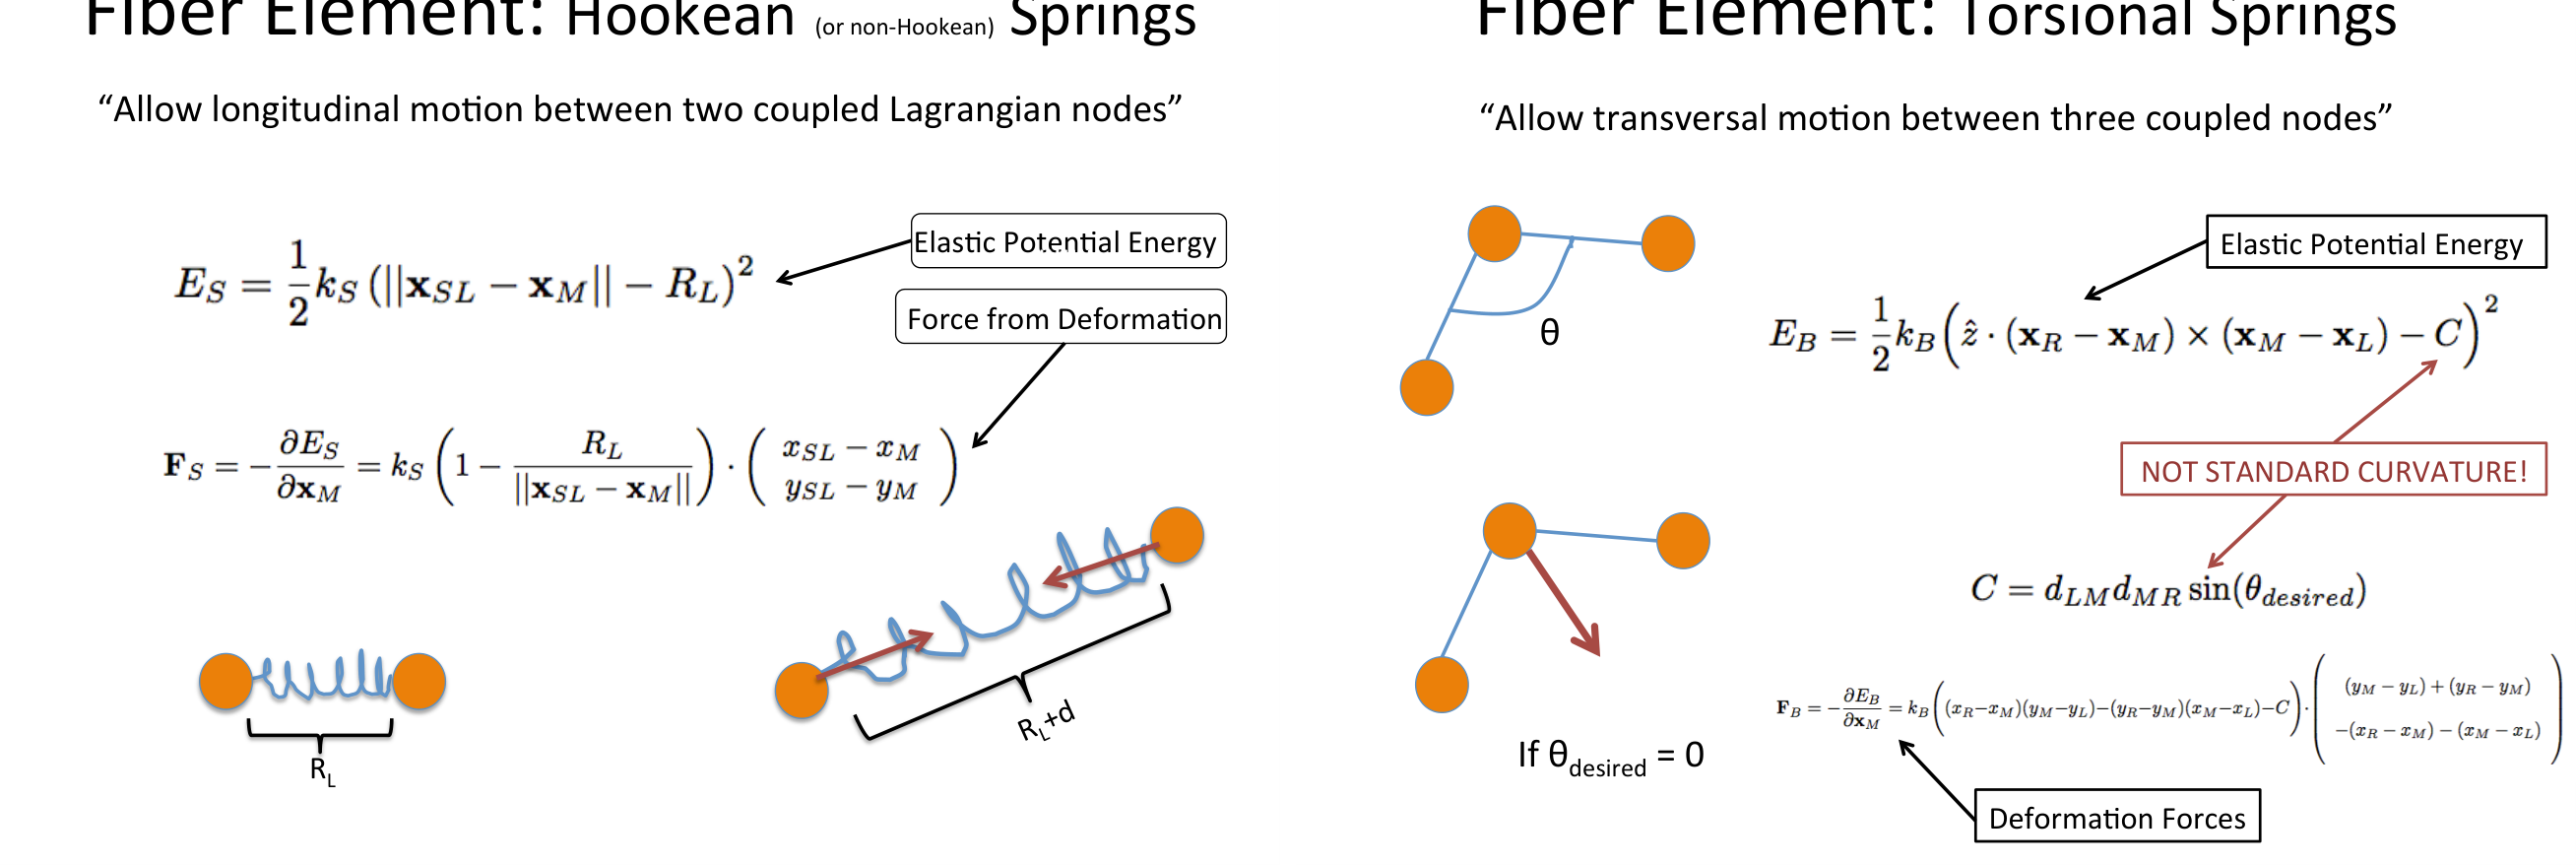
\includegraphics[width=0.86\textwidth]{ch4e-talk-springs-beams.png}

\small
Springs allow longitudinal motion between two coupled nodes; torsional springs allow transversal motion between three. The talk's warning on the right: $C = d_{LM}\,d_{MR} \sin\theta_{\text{desired}}$ is \al{not standard curvature} but a cross product of the two segments, so it depends on the spacing. Chapter 4a has both force laws as coded (springs $\tfrac12(\alpha+1)k(|d| - L)^\alpha$, torsional springs from the cross product) and runs the rubber band and the wobbly beam; chapter 4d measures the band's stiffness scaling.
\sourcecredit{The 2016 talk, pages 23 and 28 (Battista and Miller).}
\end{frame}

\begin{frame}{Non-invariant beams: \code{Wobbly\_NonInv\_Beam}}
\label{fr:noninv}
\centering
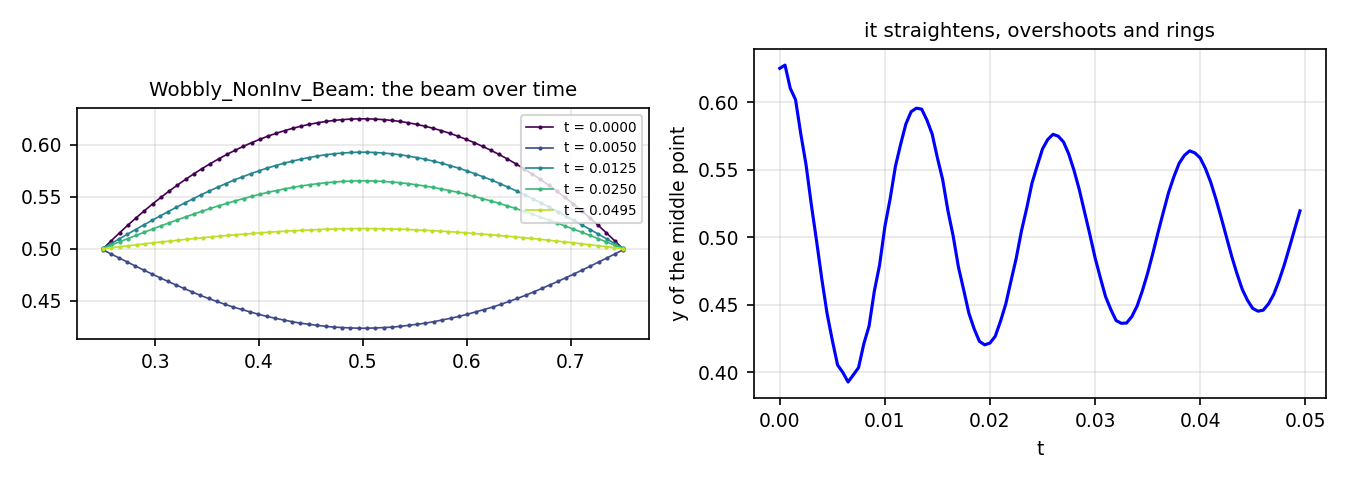
\includegraphics[width=0.66\textwidth]{ch4e-noninv-beam.png}

\scriptsize
\begin{columns}[T]
\column{0.5\textwidth}
64 points from $(0.25, 0.5)$ to $(0.75, 0.5)$, starting as an arc (middle at $y = 0.625$); 62 non-invariant beams with $k_b = 10^{10}$ and a straight rest shape ($C_x = C_y = 0$); the two end points held by target points ($k_t = 2 \cdot 10^8$); $\mu = 0.1$, $32^2$, $\Delta t = 10^{-5}$, $T = 0.05$: 5000 steps, 7.3 s.
\column{0.48\textwidth}
The beam snaps through the straight line to $y = 0.39$ at $t \approx 0.0065$, back to $0.60$, and rings with a period of about $0.013$ and a slowly shrinking amplitude (the swing narrows from 0.39--0.60 to 0.45--0.56; at the last dump, $t = 0.0495$, the middle is at 0.52, rising). ``Non-invariant'' because the rest shape is a fixed pair $(C_x, C_y)$ in the lab frame: rotate a beam with a curved rest shape and it no longer is at rest (chapter 4a, \code{.nonInv\_beam}); a straight rest shape like this one ($C_x = C_y = 0$, evenly spaced points) is at rest in any orientation.
\end{columns}
\end{frame}

% ---------------------------------------------------------------- target points
\begin{frame}{Target points: the gallery}
\label{fr:targets}
\footnotesize
A target point ties a Lagrangian node $\mathbf{x}_M$ to a virtual point $\mathbf{x}_M^T$ by a spring of zero resting length:
\[ E_T(\mathbf{x}_M) = \tfrac12 k_T\, \| \mathbf{x}_M - \mathbf{x}_M^T \|^2, \qquad \mathbf{F}_T = -\frac{\partial E_T}{\partial \mathbf{x}_M} = -k_T\,(\mathbf{x}_M - \mathbf{x}_M^T). \]
``Prescribe motion or make structure rigid'': hold the virtual points still (walls, a cylinder) or move them (chapter 4c's update function).
\begin{itemize}
  \item \al{Pulsing heart} (chapter 4c, ported and run): only target points, interpolated between two positions with a polynomial ``to avoid instantaneous accelerations''; the talk colours it by pressure.
  \item \al{Romance and dating} (\code{Example\_KC}): only target points, interpolated between \emph{three} positions to spell a message; coloured by vorticity.
  \item \al{Moving rubber band, sawtooth} (chapter 4c); \al{corals}, \al{insect flight} at $1024^2$, and every wall and cylinder in this chapter's channel examples.
\end{itemize}
The stiffness $k_T$ trades rigidity against the time step (chapter 4d: on the rubber band a stiffer spring needs a smaller step; chapter 4c: on the sawtooth pump stiffer tethers failed sooner at the same step).
\sourcecredit{The 2016 talk, pages 30--42.}
\end{frame}

% ---------------------------------------------------------------- mass
\begin{frame}{Massive points}
\label{fr:mass}
\begin{columns}[T]
\column{0.52\textwidth}
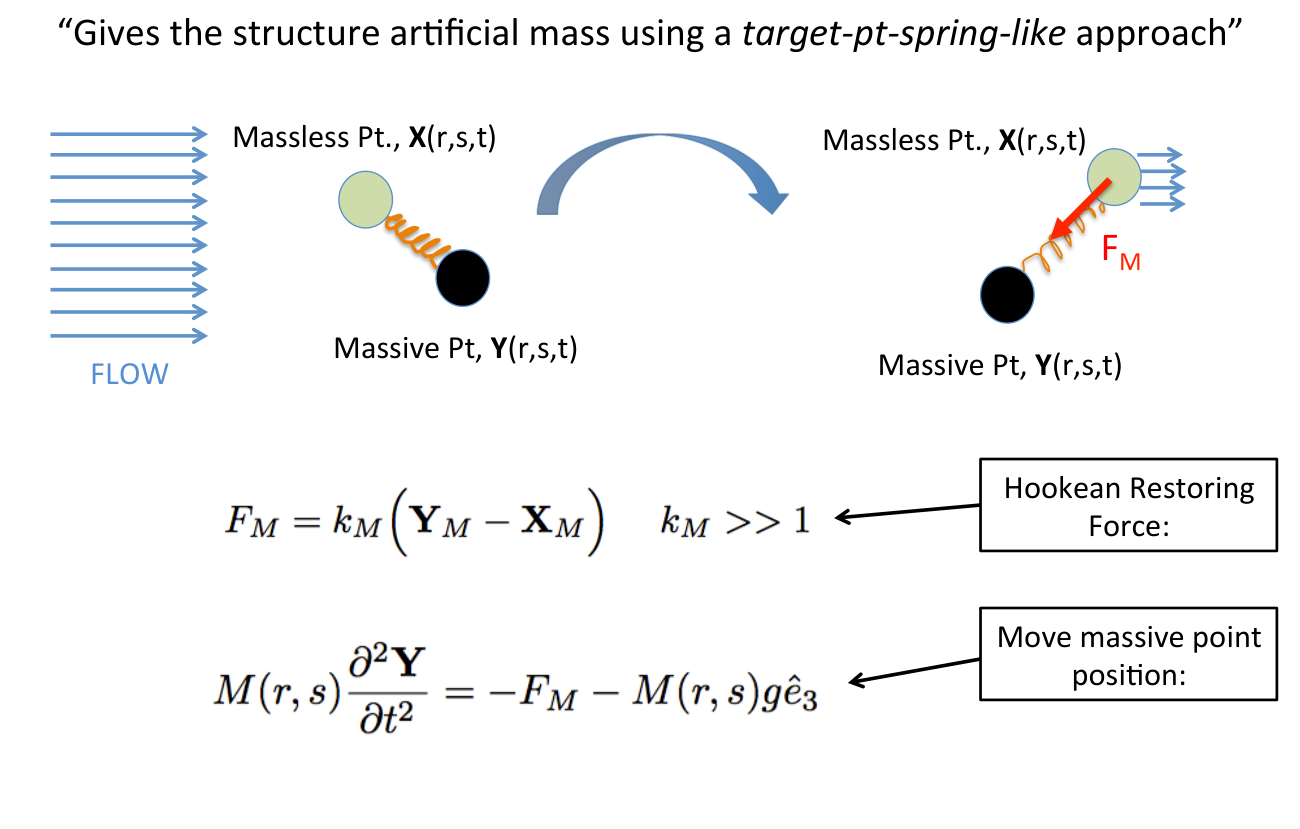
\includegraphics[width=\textwidth]{ch4e-talk-mass.png}
\sourcecredit{The 2016 talk, page 46.}
\column{0.46\textwidth}
\scriptsize
``Gives the structure artificial mass using a target-pt-spring-like approach.'' Each massless point $\mathbf{X}$ (which moves with the fluid and spreads force) has a massive twin $\mathbf{Y}$ that does not touch the fluid; a stiff spring ties them:
\[ \mathbf{F}_M = k_M\,(\mathbf{Y} - \mathbf{X}) \ \text{ on } \mathbf{X}, \qquad M\,\ddot{\mathbf{Y}} = -\mathbf{F}_M + M g\,\hat{\mathbf{g}}. \]
In the code (\code{give\_Me\_Mass\_}\allowbreak\code{Lagrangian\_Force\_Densities}, \code{please\_Update\_}\allowbreak\code{Massive\_Boundary\_Velocity}):
\begin{itemize}
  \item \code{.mass} rows are \code{index  k\_M  M}; $\mathbf{Y}$ starts on $\mathbf{X}$;
  \item $g = 9.80665$ is hard-coded; the direction $\hat{\mathbf{g}}$ is the normalised \code{(x\_gravity\_vec\_comp,}\allowbreak\code{ y\_gravity\_vec\_comp)};
  \item $M$ is a mass \al{per unit length}, like every IB2d force a density: the fluid feels $k_M(\mathbf{Y} - \mathbf{X})\,\Delta s$ with the driver's $\Delta s = L_x/(2N_x)$ (chapter 4d), so a point's weight on the fluid is $M g\,\Delta s$. The next two slides check this.
\end{itemize}
\end{columns}
\end{frame}

\begin{frame}{The gravity race: \code{Gravity\_Cellular\_Race}}
\label{fr:race}
\centering
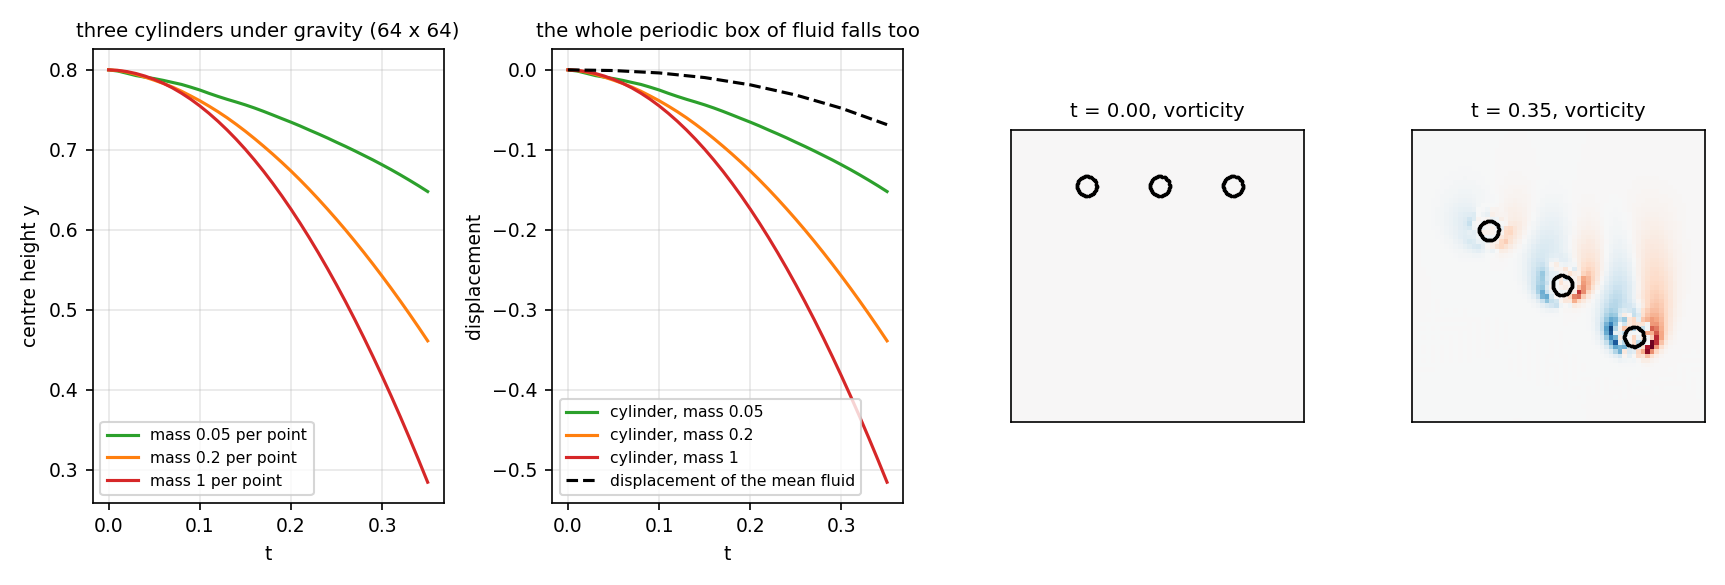
\includegraphics[width=0.94\textwidth]{ch4e-gravity-race.png}

\scriptsize
\begin{columns}[T]
\column{0.5\textwidth}
Three cylinders of 54 points (radius $1/30$, centres $(0.25, 0.8)$, $(0.5, 0.8)$, $(0.75, 0.8)$), springs $k = 5 \cdot 10^7$ and beams $k_b = 10^7$ around each (and 27 springs across each, $k = 5 \cdot 10^5$, resting length the diameter), $k_M = 10^6$, and $M = 0.05$, $0.2$ and $1$ per point; gravity $(0, -1)$; $\mu = 0.01$, $64^2$, $\Delta t = 5 \cdot 10^{-5}$, $T = 0.35$: 30 s. (The generator is called \code{Channel\_Channel.py}, but there is no channel: only the three cylinders in the periodic box.)
\column{0.48\textwidth}
At $t = 0.35$ the cylinders have fallen 0.152, 0.339 and 0.515, and are still accelerating (speeds 0.72, 1.70, 2.80). The heavier the cylinder, the stronger the wake (right). And the \al{whole box of fluid falls too}: its mean vertical velocity is $-0.45$ at $t = 0.35$ and growing (dashed line: the mean fluid's displacement).
\end{columns}
\end{frame}

\begin{frame}{Why the whole fluid falls: a momentum check}
\label{fr:momentum}
\begin{columns}[T]
\column{0.5\textwidth}
\scriptsize
\begin{tabular}{@{}rrrrr@{}}
\toprule
$t$ & fluid & masses & sum & weight $\times\, t$ \\
\midrule
0.05 & $-0.034$ & $-0.227$ & $-0.260$ & $-0.259$ \\
0.10 & $-0.086$ & $-0.433$ & $-0.519$ & $-0.517$ \\
0.15 & $-0.147$ & $-0.627$ & $-0.774$ & $-0.776$ \\
0.20 & $-0.217$ & $-0.818$ & $-1.036$ & $-1.034$ \\
0.25 & $-0.292$ & $-1.002$ & $-1.294$ & $-1.293$ \\
0.30 & $-0.368$ & $-1.183$ & $-1.552$ & $-1.551$ \\
0.35 & $-0.453$ & $-1.339$ & $-1.792$ & $-1.810$ \\
\bottomrule
\end{tabular}

\vspace{1mm}
Vertical momentum: the fluid's ($\rho \times$ mean $u_y \times$ box area) plus the cylinders' ($\sum 54\,M\,\Delta s \times$ the centre's speed), against the total weight $\sum 54\,M g\,\Delta s = 5.17$ times $t$.
\column{0.48\textwidth}
\scriptsize
The two columns agree to 0.5\,\% until $t = 0.30$ (1\,\% at $0.35$, the last dump, where the speeds are one-sided differences): Newton's second law for fluid plus cylinders, with the weight $M g\,\Delta s$ per point. That confirms the per-unit-length reading of $M$ and $\Delta s = L_x/(2N_x)$.
\begin{itemize}
  \item In a \al{periodic box} nothing holds the weight up: no walls, no bottom. The pressure of a periodic solver has no mean gradient, so the whole fluid accelerates with the cylinders. ``Terminal velocity'' never comes.
  \item For a settling problem, put walls in (target points: the MATLAB \code{Gravity\_vs\_Flow} and \code{Channel\_Flow\_Cellular\_Race} run in channels, but the MATLAB \code{Gravity\_Cellular\_Race}, like the Python one, has none), or subtract the mean force from the fluid each step (the option \code{balance\_periodic\_force} of the \code{python-updates-2026} branch, pull request 34 to IB2d) and measure speeds relative to the fluid.
\end{itemize}
\end{columns}
\end{frame}

\begin{frame}{\code{Thrips}, and the MATLAB races}
\label{fr:thrips}
\begin{columns}[T]
\column{0.42\textwidth}
\footnotesize
\al{\code{Thrips}:} one massive point at $(0.25, 0.4113)$ in a $0.5 \times 0.5$ box, gravity on, $\mu = 0.1$, $32^2$, $T = 0.1$. It falls $1.1 \cdot 10^{-5}$ in 0.1 time units (speed $1.7 \cdot 10^{-4}$ at the end), where free fall would be $0.049$: its weight on the fluid is $M g\,\Delta s = 0.001 \times 9.807 \times 0.0078 = 7.7 \cdot 10^{-5}$. The folder is a stub: \code{make2d.py} would write $k_M = 10^6$, $M = 6 \cdot 10^{-8}$, but the shipped \code{thrips.mass} holds $k_M = 1000$, $M = 0.001$ (and a second geometry, \code{thrips2.*}, is unused).
\column{0.56\textwidth}
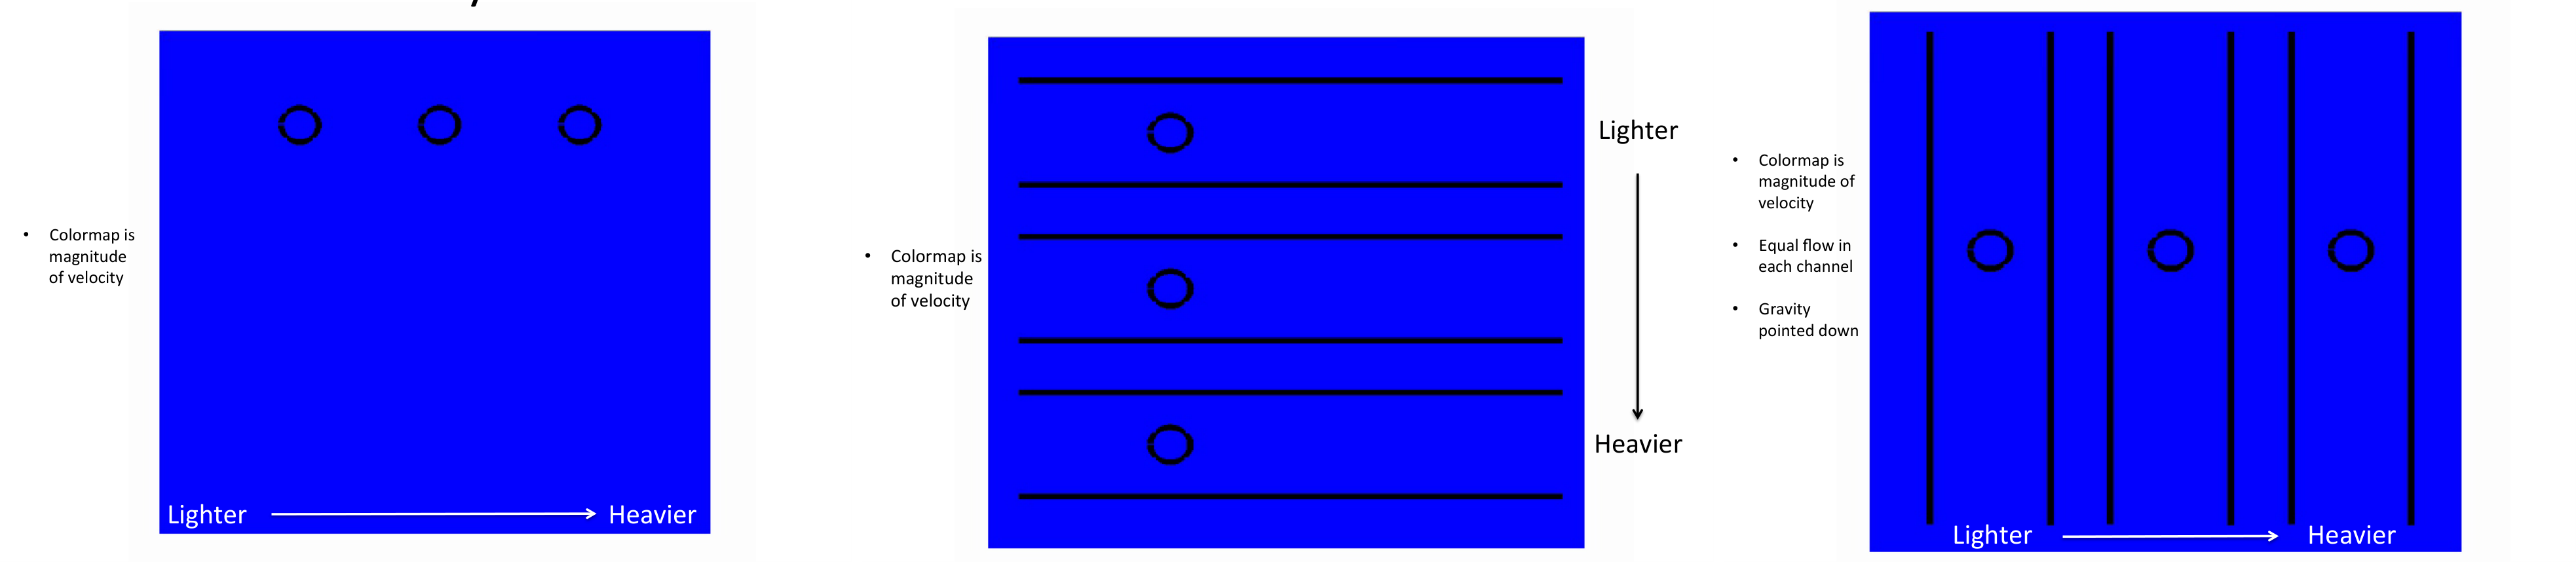
\includegraphics[width=\textwidth]{ch4e-talk-races.png}
\scriptsize
The MATLAB races of the 2016 talk (set-ups, first frames): ``Mass vs.\ gravity cell race'', ``Channel flow mass race'', ``Mass--gravity--flow race'' (equal flow in each channel, gravity down); colour is the speed. \code{Example\_Mass\_Points/Gravity\_Cellular\_Race}, \code{Channel\_Flow\_Cellular\_Race}, \code{Gravity\_vs\_Flow}.
\end{columns}
\sourcecredit{The 2016 talk, pages 47, 48 and 54.}
\end{frame}

% ---------------------------------------------------------------- artificial velocity, channels
\begin{frame}[fragile]{Artificial velocity: an external force on the grid}
\label{fr:artvel}
\begin{columns}[T]
\column{0.5\textwidth}
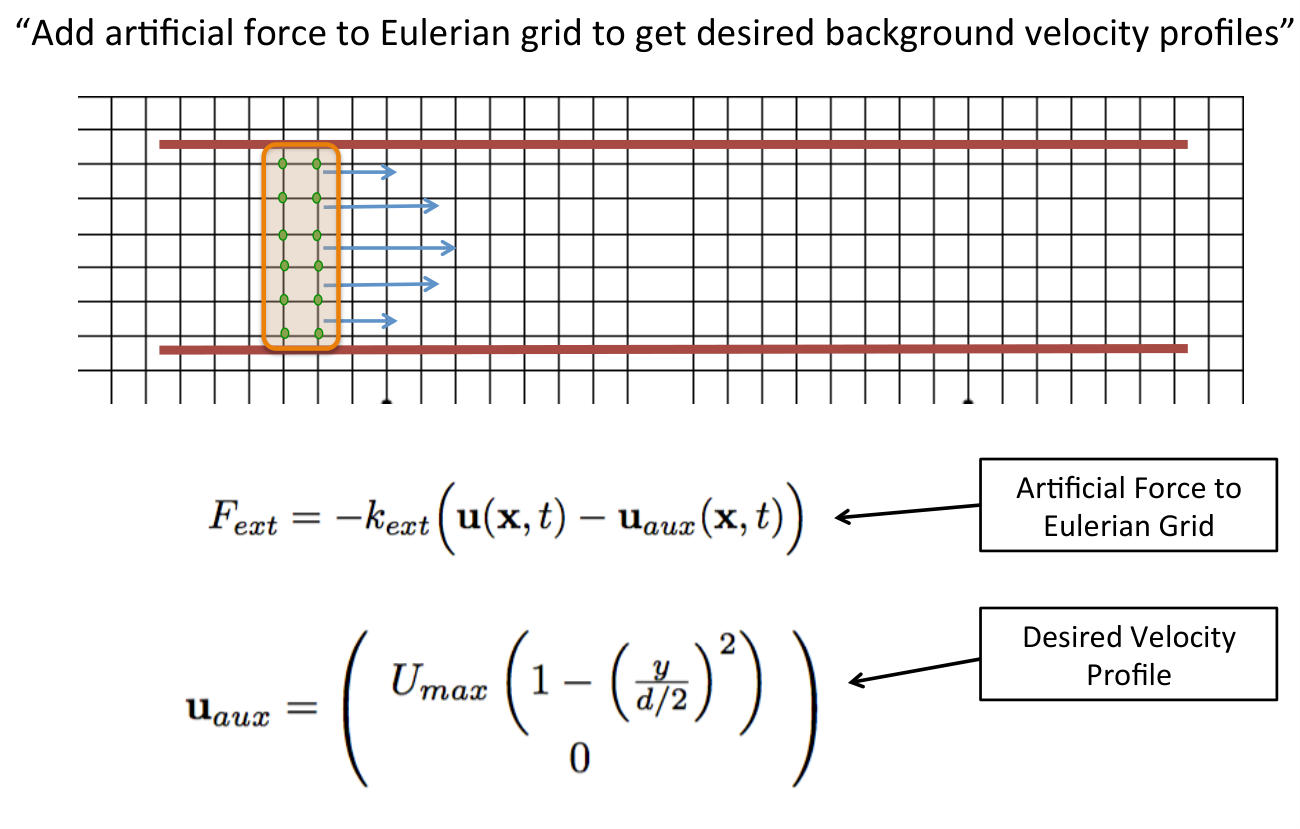
\includegraphics[width=\textwidth]{ch4e-talk-artvel.png}
\sourcecredit{The 2016 talk, page 52.}
\column{0.48\textwidth}
\footnotesize
``Add artificial force to Eulerian grid to get desired background velocity profiles'': in a box of grid cells, a penalty force pulls the fluid towards a target velocity,
\[ \mathbf{F}_{\text{ext}} = -k_{\text{ext}}\,\big(\mathbf{u}(\mathbf{x}, t) - \mathbf{u}_{\text{aux}}(\mathbf{x}, t)\big), \]
with a parabolic $\mathbf{u}_{\text{aux}}$ across the channel. The example supplies \code{please\_Compute\_External\_Forcing.py} and sets \code{arb\_ext\_force = 1}; in \code{Turek\_Hron} the box is $0.1 \le x \le 0.16$, $0.035 \le y \le 0.215$ and
\begin{lstlisting}[style=pytiny]
uX_Tar = -Umax * (100 * np.tanh(2*t)) * ( (Ly/2+w/2) - y ) * ( (Ly/2-w/2) - y )
fx[j,i] = fx[j,i] - kStiff*( uX[j,i] - uX_Tar )
\end{lstlisting}
($U_{\max} = 2.75$, $w = 0.2$, $L_y = 0.25$, $k = 10^3$): a parabola that vanishes at the walls $y = 0.025$ and $0.225$, peaks at $2.75\tanh 2t$ on the centre line, and ramps up over $t \sim 0.5$.
\end{columns}
\end{frame}

\begin{frame}{Channel flows, and the bifurcating artery}
\label{fr:channels}
\begin{columns}[T]
\column{0.46\textwidth}
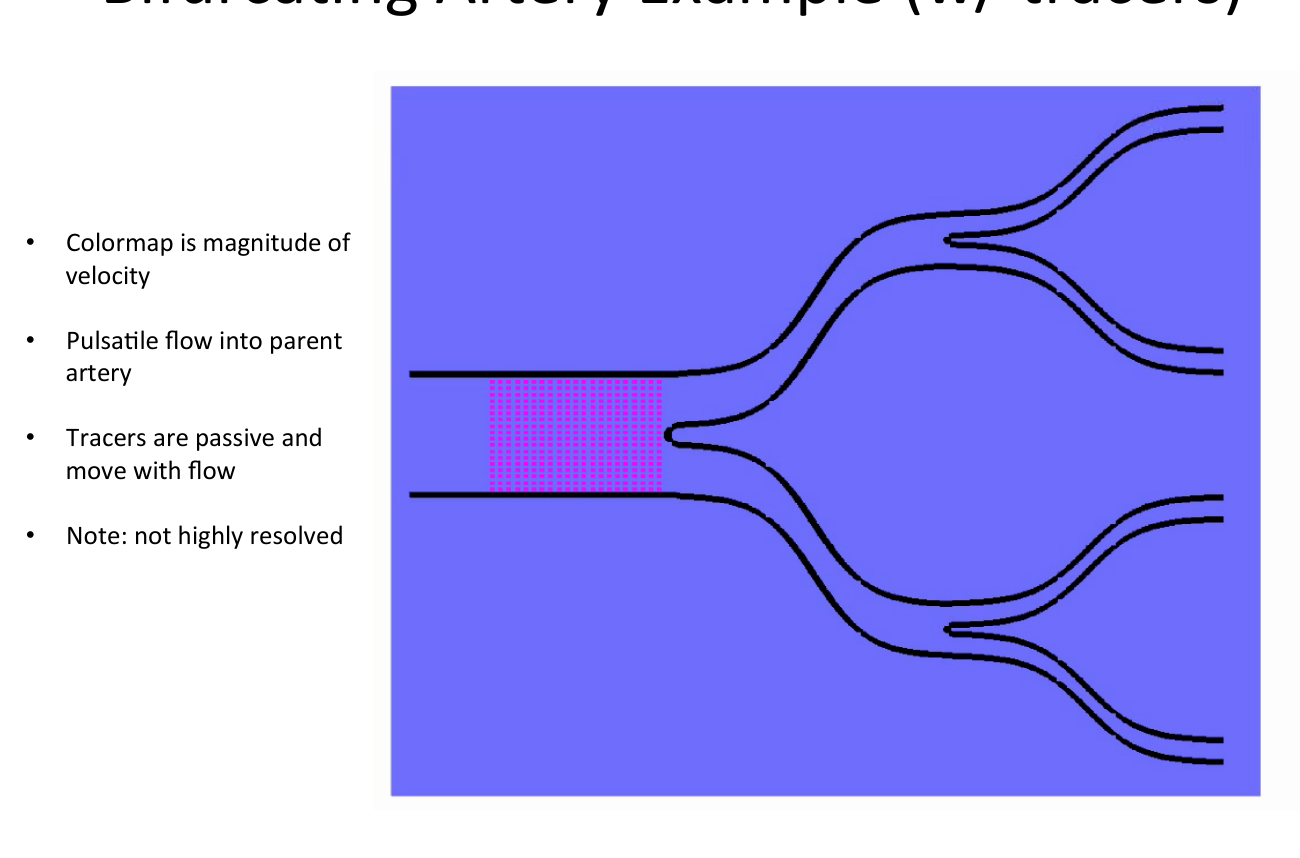
\includegraphics[width=\textwidth]{ch4e-talk-artery.png}
\sourcecredit{The 2016 talk, page 53: \code{Example\_Tracers/Tracers\_In\_Bifurcating\_Artery}.}
\column{0.52\textwidth}
\footnotesize
\al{Bifurcating artery with tracers:} pulsatile flow into the parent artery from an external force, passive tracers that move with the flow, colour the speed; ``not highly resolved''.

\al{\code{Example\_Channel\_Flow}:} the same forcing makes every channel flow of IB2d: around a cylinder between two walls or next to one, through a hole in the wall, in the middle of the domain, in an empty channel, in an aneurysm, past a cylinder with a flag (Turek--Hron, next slide), through a Brinkman medium, past a poroelastic obstacle, carrying a concentration (the bifurcating artery of \code{Example\_Concentration\_Gradients}; its other two are not forced).

Three things to know: the walls are target points (there are no wall boundary conditions in a periodic code); what leaves the right edge comes back in at the left, so the forcing box also has to remove the wake; and the force is a penalty, so the velocity in the box only approaches the target, as closely as the stiffness $k$ allows.
\end{columns}
\end{frame}

\begin{frame}{\code{Turek\_Hron}: a flag behind a cylinder}
\label{fr:th}
\centering
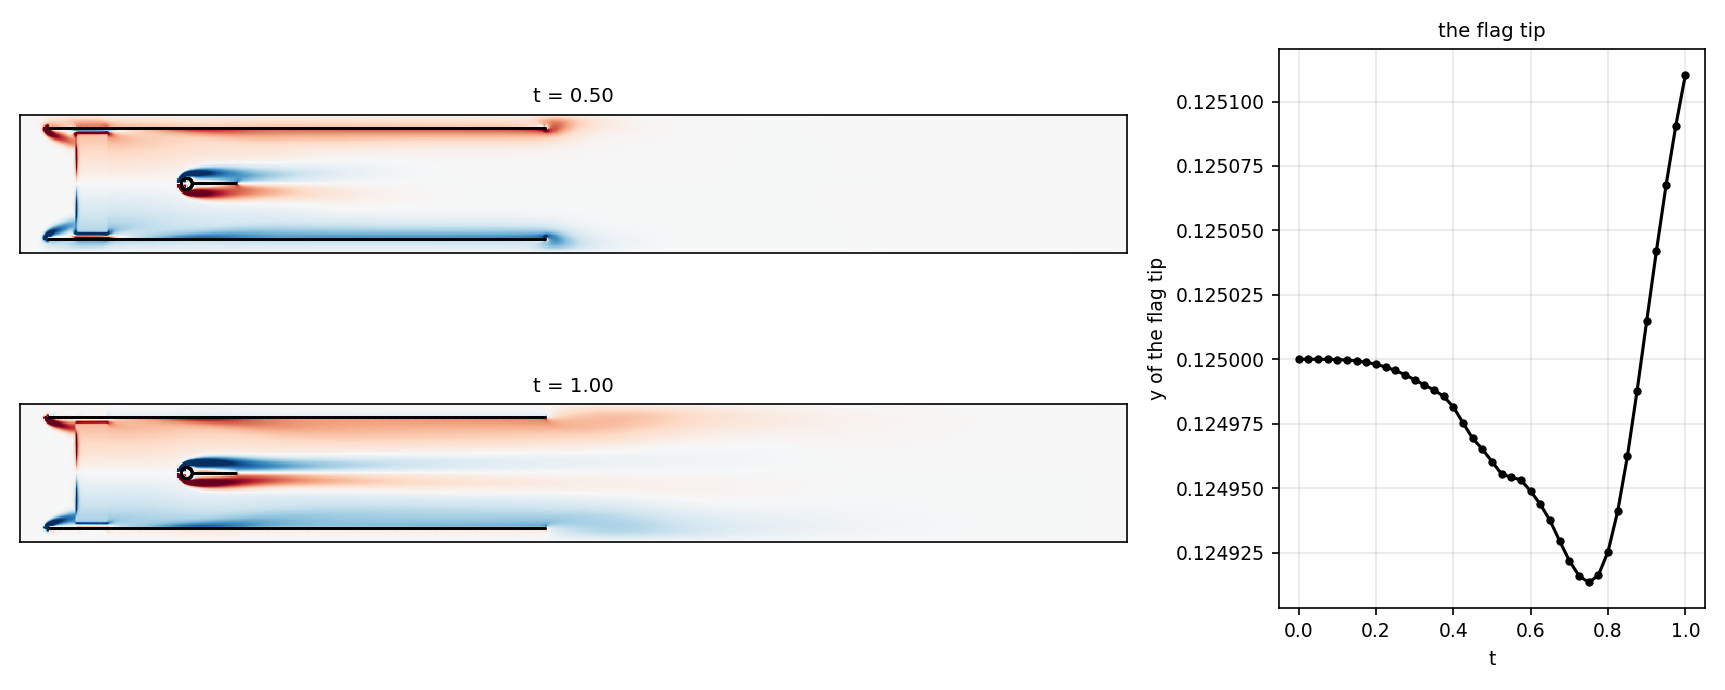
\includegraphics[width=0.78\textwidth]{ch4e-turek-hron.png}

\scriptsize
\begin{columns}[T]
\column{0.5\textwidth}
A $2 \times 0.25$ periodic box, $1024 \times 128$; a channel of target-point walls at $y = 0.025$ and $0.225$ from $x = 0.05$ to $0.95$ (the right half of the box is open fluid, where the wake leaves the channel); a cylinder of radius 0.01 at $(0.30, 0.125)$, held by target points; a flag of 80 points from $x = 0.313$ to $0.390$ (springs, beams, mass $M = 5$ per point); the forcing box of slide \ref{fr:artvel} at the inlet. Walls and cylinder points carry mass as well as targets. $\mu = 7.5 \cdot 10^{-4}$, $\Delta t = 5 \cdot 10^{-5}$; run to $T = 1$ (shipped: 8): 20\,000 steps, 21 minutes.
\column{0.48\textwidth}
Vorticity at $t = 0.5$ and $1$: shear layers on the walls and the cylinder, the forcing box (the rectangle at the inlet), the jet leaving the channel at $x = 0.95$. By $t = 1$ the flag tip has moved by $10^{-4}$ (right): the inflow has only just reached full speed ($2.75\tanh 2t$), and the flapping the benchmark measures needs more time (the shipped run goes to $t = 8$). The proportions are not the benchmark's (Turek and Hron: channel $4.1D$ wide, flag $3.5D$ long; here $10D$ and $3.9D$), so compare shapes, not numbers.
\end{columns}
\end{frame}

% ---------------------------------------------------------------- porous
\begin{frame}{Porous points}
\label{fr:porous}
\begin{columns}[T]
\column{0.4\textwidth}
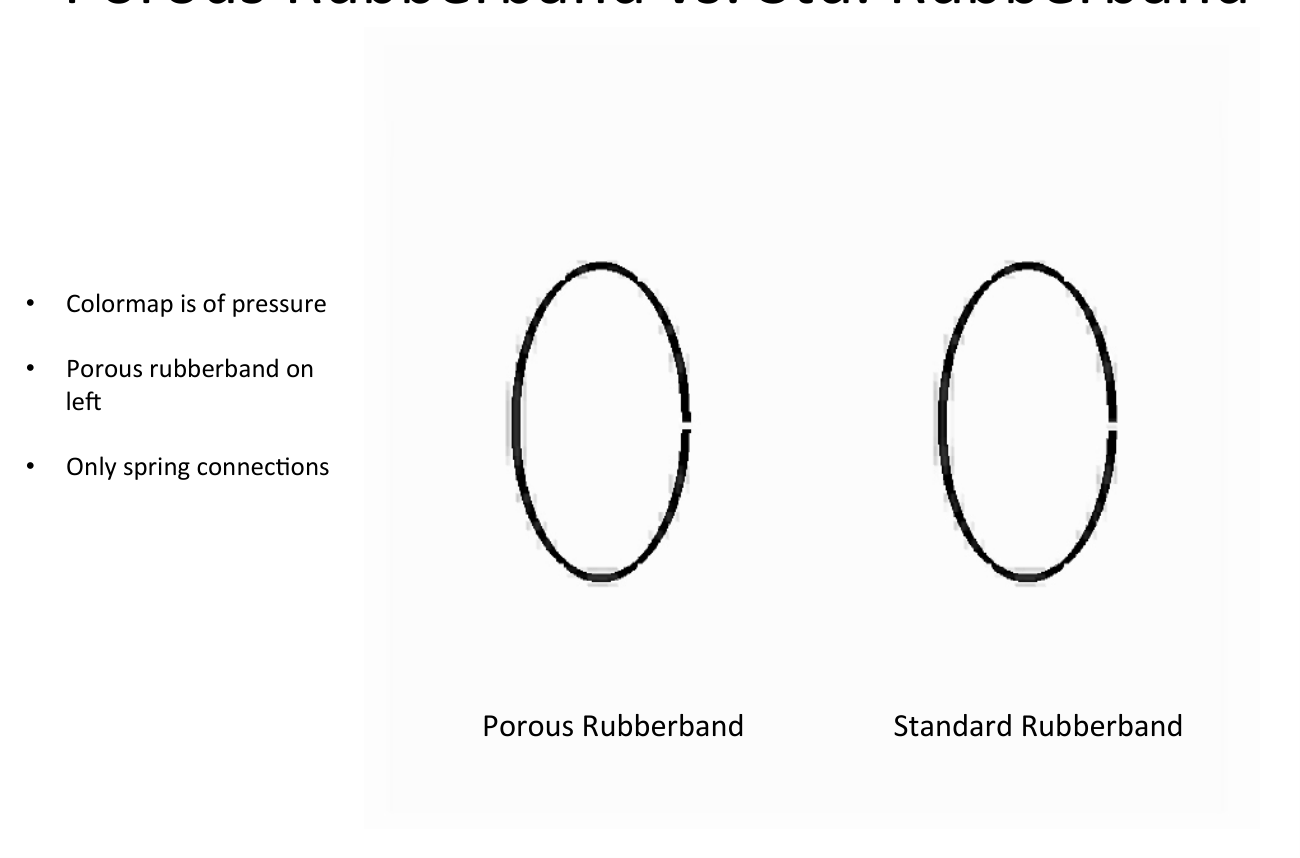
\includegraphics[width=\textwidth]{ch4e-talk-porous.png}
\sourcecredit{The 2016 talk, page 59: a porous band (left) and a standard band, coloured by pressure.}
\column{0.58\textwidth}
\scriptsize
``Makes the structure permeable to fluid flowing through it.'' Darcy's law gives the slip of the fluid through the membrane relative to the boundary,
\[ U_p\,\hat{\mathbf{n}} = -\frac{\kappa\,[p]}{\mu\,a} \qquad (\kappa \text{ permeability}, a \text{ thickness}, [p] \text{ pressure jump}), \]
and the boundary moves with the fluid velocity plus the slip. In IB2d the pressure jump is the boundary's own force: \code{please\_Compute\_}\allowbreak\code{Porous\_Slip\_Velocity} sets
\[ U_{p,x} = -\kappa_i\,F_x\,n_x/|\mathbf{X}_s|, \qquad U_{p,y} = -\kappa_i\,F_y\,n_y/|\mathbf{X}_s|, \]
with the normal from a five-point derivative along the band. \code{.porous} rows are \code{index kappa stencil}, the last column ($-2 \ldots 2$) saying where the point sits in the stencil (ends of open structures). The talk notes ``only spring connections'' in its picture.

\al{Poroelastic points} (\code{.poroelastic}: \code{index alpha}) add a second drift: each listed point moves by $\Delta t\,\mathbf{F}_{\text{spring}}/(\mu\,\alpha)$ every step (\code{Supp.py}, lines 116--122; the file calls $\alpha$ a ``Brinkman constant'').
\end{columns}
\end{frame}

\begin{frame}{The porous bands, run past their end time}
\label{fr:porousrun}
\centering
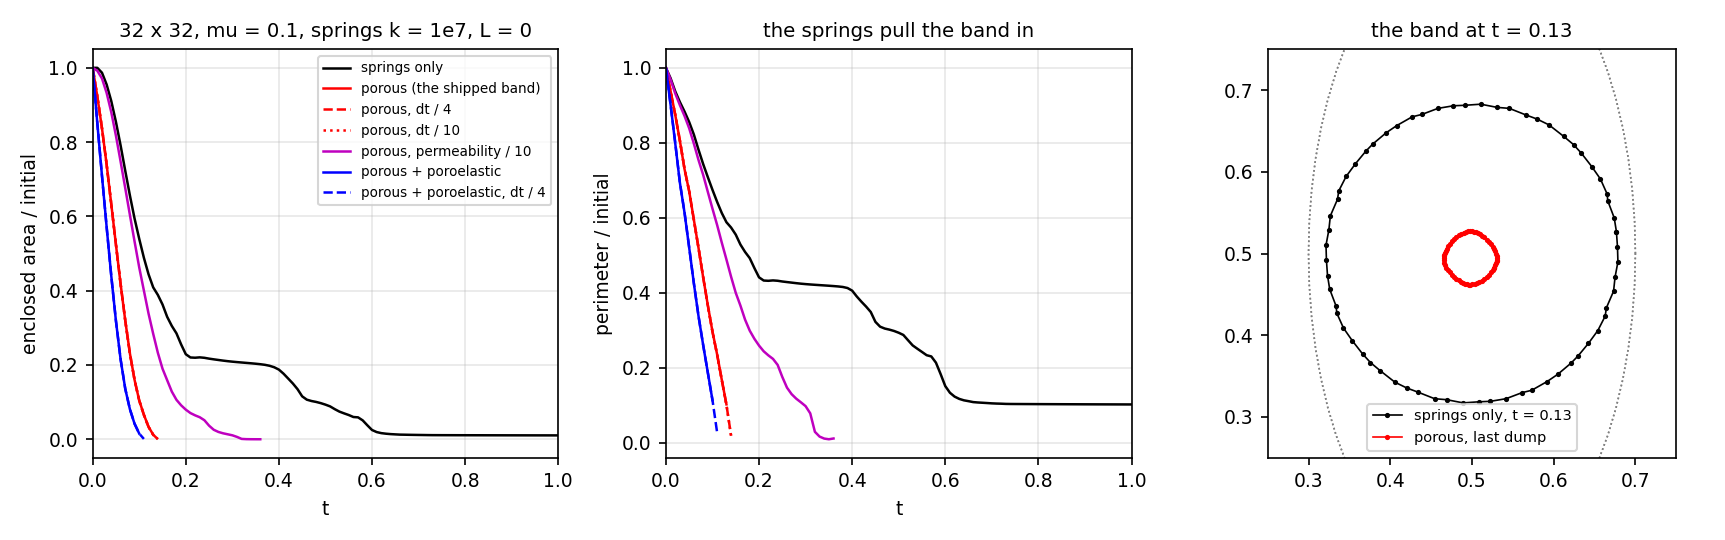
\includegraphics[width=0.92\textwidth]{ch4e-porous-bands.png}

\raggedright\small
Both shipped bands are stiff: 64 points, springs $k = 10^7$, resting length 0, $\mu = 0.1$, $32^2$, $\Delta t = 10^{-4}$, and they stop at $T = 0.1$. Run to $T = 1$: the band without porosity keeps 54\,\% of its area at $t = 0.1$, 23\,\% at $0.2$, 2.5\,\% at $0.6$ and 1\,\% from $t \approx 0.7$ on (the method's volume loss, chapter 4d, at a tension 400 times the standard band's); the porous band keeps 10\,\% at $t = 0.1$ and stops at $t = 0.13$; the poroelastic band stops at $t = 0.10$. Why they stop: next slide.
\end{frame}

\begin{frame}{Why the porous bands stop}
\label{fr:porousstop}
\small
\begin{itemize}
  \item The stops are not a time-step problem: at $\Delta t / 4$ and $\Delta t / 10$ the porous band stops at $t = 0.14$, and at $\Delta t / 4$ (the only smaller step tried for it) the poroelastic at $0.11$; their area curves lie on those at $\Delta t$.
  \item With the permeability divided by ten it lasts to $t = 0.36$.
  \item Each time the band has \al{collapsed} by its last dump (area 0--1.5\,\% of the start, perimeter 1--11\,\%, closest neighbours $5 \cdot 10^{-5}$ to $3 \cdot 10^{-3}$ apart, a seven-hundredth to an eleventh of a cell): springs of zero resting length pull a porous band to a point, where the code divides by distances that vanish (the spring directions, and the porous slip's $|\mathbf{X}_s|$; which fails first was not traced), and the run ends with chapter 4d's \code{IndexError} (all six logs).
  \item The sealed band is at area 1\,\%, perimeter 10\,\% and neighbours $5 \cdot 10^{-4}$ apart by $t = 1$, and runs on. The shipped $T = 0.1$ ends just before.
\end{itemize}
\end{frame}

% ---------------------------------------------------------------- concentration, Boussinesq
\begin{frame}{A concentration: \code{Concentration\_Diffusion}}
\label{fr:conc}
\centering
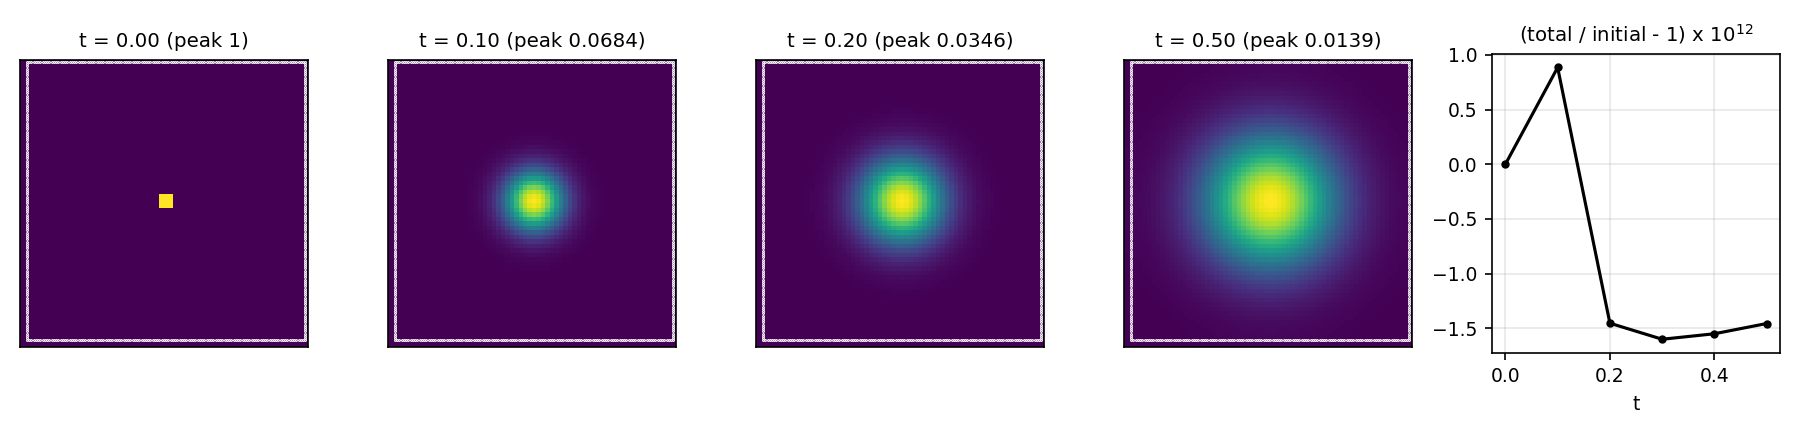
\includegraphics[width=0.96\textwidth]{ch4e-concentration.png}

\footnotesize
\begin{columns}[T]
\column{0.5\textwidth}
\code{concentration = 1} reads \code{<name>.concentration}: its first line is the diffusion coefficient (here $0.025$), then the initial field on the grid ($N_y$ rows of $N_x$ values). The driver advects and diffuses it with the flow every step. Here: a $3 \times 3$-cell square of $C = 1$ in the middle of a box walled by target points ($k = 10^7$), $\mu = 10$ (and no flow at all: $|\mathbf{u}| = 0$ in every saved velocity field), $64^2$, $T = 0.5$: 32 s.
\column{0.48\textwidth}
The peak falls from 1 to 0.068 at $t = 0.1$ and 0.014 at $t = 0.5$; the spread grows like $\sqrt{2Dt}$ ($0.16$ at $t = 0.5$). The total amount $\sum C\,\Delta x\,\Delta y = 0.002197$ is conserved to $2 \cdot 10^{-12}$ of itself (right): with the fluid at rest only the diffusion part acts, and it conserves; the cheapest check of a concentration run (slide \ref{fr:rt2}: the upwind advection fails it once the fluid moves). A \code{source} flag and the \code{Example\_Concentration\_Dynamics} folders (corals, a leaf, a sink) add production and uptake in MATLAB.
\end{columns}
\end{frame}

\begin{frame}{Buoyancy: \code{Rayleigh\_Taylor\_Instability}}
\label{fr:rt}
\centering
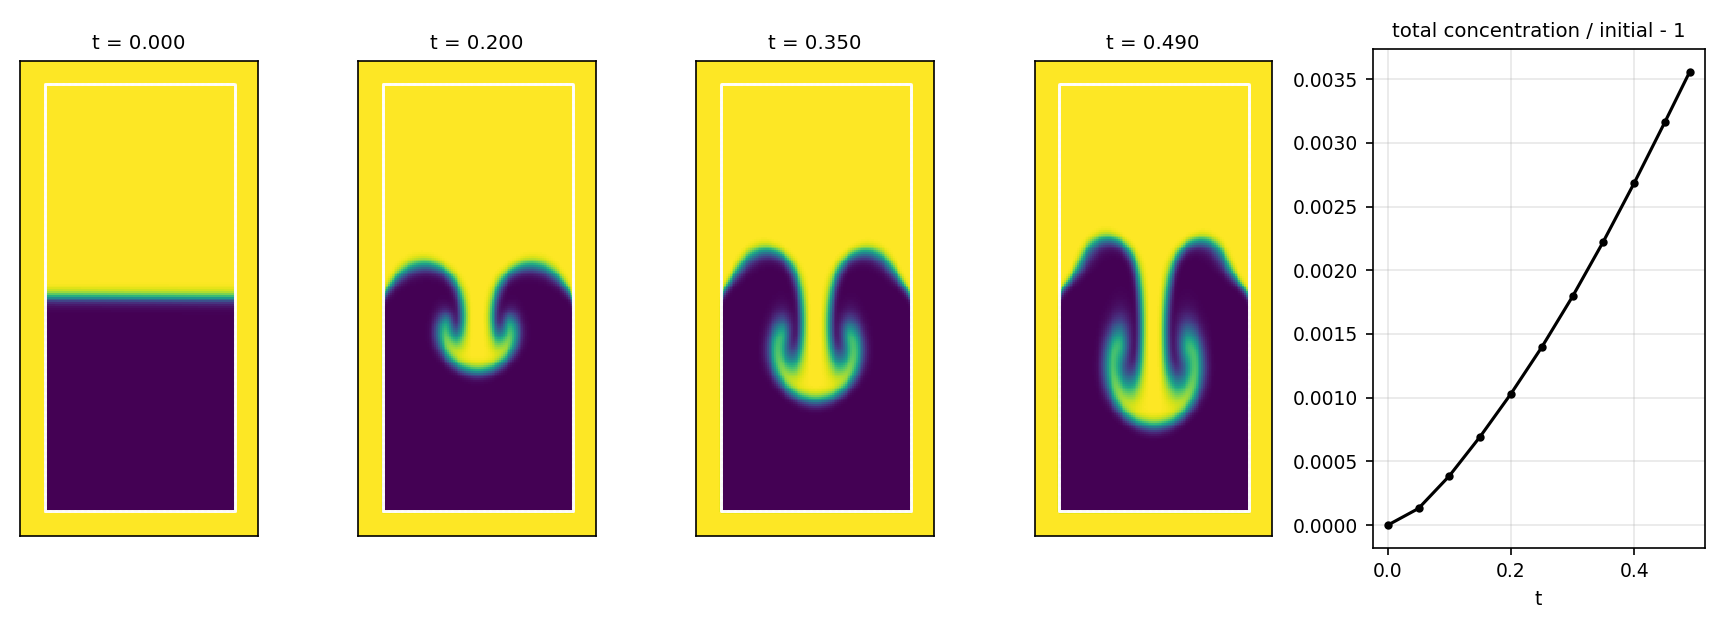
\includegraphics[width=0.84\textwidth]{ch4e-rayleigh-taylor.png}

\footnotesize
A $0.5 \times 1$ box, $128 \times 256$, holding a tub of 2660 target points ($0.05 \le x \le 0.45$, $0.05 \le y \le 0.95$); a concentration $C = 1$ (heavy) above $y = 0.5$ in the tub and outside it, $C = 0$ (light) below. \code{boussinesq = 1} adds the force $\rho\,\beta\,g\,C\,\hat{\mathbf{g}}$ on the 23\,793 grid cells listed in \code{boussinesq.mesh} (the inside of the tub), with $\beta =$ \code{expansion\_coeff} $= 10$ and $g = 0.981$ written into the example's own \code{please\_Form\_Boussinesq\_Forcing\_Terms.py} (not the 9.80665 of the mass points). $\mu = 0.01$, $\Delta t = 1.25 \cdot 10^{-5}$; run to $T = 0.5$ (shipped: 2): 40\,000 steps, 29 minutes.
\end{frame}

\begin{frame}{Buoyancy, continued: a seeded plume, and a scheme that does not conserve}
\label{fr:rt2}
\small
The mushroom at $t = 0.49$ is \al{seeded}, not driven: the example also sets \code{arb\_ext\_force = 1}, and its \code{please\_Compute\_External\_Forcing.py} pulls the fluid in the box $0.2 \le x \le 0.3$, $0.48 \le y \le 0.52$ (the middle of the interface) towards $u_y = -10\tanh 20t$ with $k = 10^4$, but only while $t < 0.01$ (\code{if (t<0.01):}, the first 800 steps; the target has then reached only $-10\tanh 0.2 \approx -2$): a short downward kick at the middle of the interface that seeds one plume, which buoyancy then grows. The total concentration is \emph{not} conserved here: it rises by $0.36\,\%$ by $t = 0.49$ (right). The scheme is first-order upwind in advective form, $C \leftarrow C + \Delta t\,(k\,C_{xx} - u\,C_x)$, split in $x$ and $y$ (\code{Supp.py}, \code{perform\_Time\_Split\_Upwind}), which conserves the total when the fluid is at rest (slide \ref{fr:conc}) but not in a flow that varies in space (a uniform flow would conserve it too, were it not for the loops below). And its Python loops stop one cell short: \code{range(1, lenX-2)} skips the column \code{lenX-2} (MATLAB's \code{for j=2:lenX-1} does not), likewise the row \code{lenY-2}, so nothing is advected there (in this run both lie outside the tub, at $x = 0.492$ and $y = 0.992$, where $C = 1$ stays uniform, so the skip is not what adds the 0.36\,\%).
\begin{punchbox}
\small Two lessons for any example you take from a gallery: read every flag that is on and the function behind it (here \code{arb\_ext\_force}, whose forcing switches itself off at $t = 0.01$), and check the conserved quantities (here the total concentration) before you read the picture.
\end{punchbox}
\end{frame}

% ---------------------------------------------------------------- user-defined
\begin{frame}[fragile]{A force law of your own: \code{User\_Defined\_Fiber\_Model}}
\label{fr:user}
\begin{columns}[T]
\column{0.55\textwidth}
\begin{lstlisting}[style=pytiny]
def give_Me_General_User_Defined_Force_Densities(ds,Nb,xLag,yLag,
            xLag_P,yLag_P,dt,current_time,general_force):
    Nsprings = general_force.shape[1]  # # of Force Connections
    id_Master = general_force[0,:].astype('int')
    id_Slave = general_force[1,:].astype('int')
    K_Vec = general_force[2,:]  # spring stiffness
    RL_Vec = general_force[3,:] # spring resting length
    fx = np.zeros(Nb); fy = np.zeros(Nb)
    dx = xLag[id_Slave] - xLag[id_Master]
    dy = yLag[id_Slave] - yLag[id_Master]
    sF_x = K_Vec * (np.sqrt(dx**2 + dy**2)-RL_Vec) * (dx/np.sqrt(dx**2+dy**2))
    sF_y = K_Vec * (np.sqrt(dx**2 + dy**2)-RL_Vec) * (dy/np.sqrt(dx**2+dy**2))
    for ii in range(Nsprings):
        fx[id_Master[ii]] += sF_x[ii]; fy[id_Master[ii]] += sF_y[ii]
        fx[id_Slave[ii]] -= sF_x[ii];  fy[id_Slave[ii]] -= sF_y[ii]
    return (fx, fy)
\end{lstlisting}
\scriptsize The example's \code{give\_Me\_General\_User\_Defined\_Force\_Densities.py}, comments shortened. The driver reads \code{rubberband.user\_force} (rows \code{i j k L}) transposed: one column per connection.
\column{0.43\textwidth}
\footnotesize
\code{user\_force\_model = 1}: the driver imports this function from the example's folder every step, passes the current and previous positions, $\Delta t$ and the time, and adds the forces it returns to all the others. Anything you can compute from the points goes here: a contact force, a nonlinear membrane, an anisotropic law.

The example's law is a Hookean spring, $k = 2.5 \cdot 10^4$, $L = 0$, on the standard rubber band: the run (1500 steps, 3.9 s) is \al{identical to the last digit} to the springs run of chapter 4d at dumps 0, 10, 25, 50 and 75. That is how to test a new law: first reproduce a built-in one exactly, then change it.
\end{columns}
\end{frame}

\begin{frame}{What else ships, briefly}
\label{fr:else}
\footnotesize
\begin{itemize}
  \item \al{Damped springs} (\code{.d\_spring}: \code{i j k L b}): a spring plus a damping force on the leader's velocity (chapter 4a ran \code{Rubberband\_with\_Damped\_Springs}); used to tether the cylinder in two of the seven \code{Example\_VIV\_Cylinder} folders (\code{Single\_VIV\_Cylinder\_Damped\_Springs\_256} and \code{\_High}, $b = 5$ and $50$), and for all 153 springs of \code{Scallop\_3Elem\_Muscle} (along and across its shell, with $b = 0$: no damping).
  \item \al{Electrophysiology} (\code{electro\_phys}, MATLAB): a FitzHugh--Nagumo excitable medium along a heart tube whose potential sets the stiffness of the tube's springs, $(16V)^4$ (\code{IBM\_Driver.m}, line 800; \code{Example\_HeartTube/Electromechanical\_Pumping*}), or, with \code{FV\_LT\_muscle = 1}, drives the muscles (\code{EM\_Pump\_w\_Calcium\_and\_Muscles}); in the folders with calcium, the stimulus is $0.5\,Caf(t)$ from a calcium model (\code{Calcium\_Dynamics.m}).
  \item \al{Brinkman} (\code{brinkman}): a drag $-\mu\,B\,\mathbf{u}$ added to the fluid force where the field $B$ (an inverse permeability, though the code calls it the permeability matrix; read from a file, written to \code{viz\_IB2d}) is non-zero; \code{Example\_Brinkman\_Channel}.
  \item \al{Coagulation} (\code{coagulation}, MATLAB): a coagulation model in a channel, stirred or tested through boundaries (\code{Example\_Coagulation}).
  \item \al{Restart} (\code{Restart\_Flag}, MATLAB): \code{Example\_Test\_Restart\_Protocol} restarts a standard and a poroelastic band from saved data.
  \item \al{Tracers} (chapter 4b): passive points that move with the flow and exert no force (\code{.tracer}); the Python tracer call needed a fix (pull request 34).
\end{itemize}
\end{frame}

% ================================================================ MUSCLES
\begin{frame}{Part 2: muscle models}
\label{fr:musclesintro}
\small
The 2015 lecture's outline, extended by the activation tutorial:
\begin{enumerate}
  \item A simple muscle model that describes the force produced as a function of the muscle fibre's \al{length and velocity} (the model IB2d's \code{FV\_LT\_muscle} uses).
  \item The \al{three-element Hill model} (contractile, series and parallel elements; IB2d's \code{3\_element\_muscle}).
  \item A \al{microscale model} of crossbridge formation and detachment, from which Hill's force--velocity law follows.
  \item \al{Activation}: from the motor neuron to calcium, force summation, and a calcium model that turns a stimulus train into the activation that multiplies the force.
\end{enumerate}
Then IB2d's muscle code: what the heart tube does, what it computes that the models do not say, and what is broken.
\begin{punchbox}
\small A muscle in IB2d is a force between two points, along the line joining them, whose size depends on their distance (length), how fast that distance changes (velocity), and an activation you write as a function of time and position. Everything below is about choosing those three.
\end{punchbox}
\end{frame}

\begin{frame}{The sarcomere and the sliding filaments}
\label{fr:sarcomere}
\begin{columns}[T]
\column{0.5\textwidth}
\centering
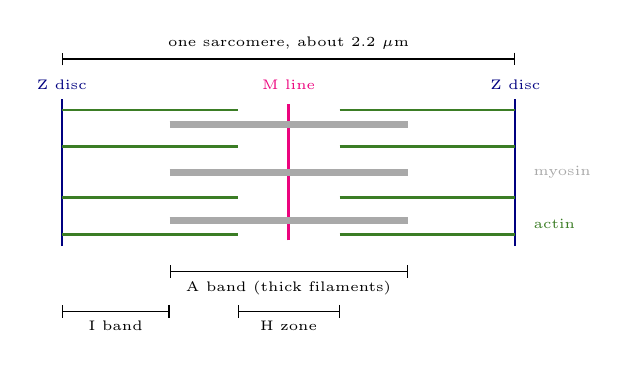
\begin{tikzpicture}[scale=0.72]
  \draw[thick,NavyBlue] (0,0) -- (0,2.6); \draw[thick,NavyBlue] (8,0) -- (8,2.6);
  \node[font=\tiny,NavyBlue] at (0,2.85) {Z disc}; \node[font=\tiny,NavyBlue] at (8,2.85) {Z disc};
  \draw[RubineRed,very thick] (4,0.1) -- (4,2.5); \node[font=\tiny,RubineRed] at (4,2.85) {M line};
  \foreach \y in {0.45,1.3,2.15} {\draw[line width=2.6pt,DarkGray] (1.9,\y) -- (6.1,\y);}
  \foreach \y in {0.2,0.85,1.75,2.4} {\draw[line width=1pt,OliveGreen] (0,\y) -- (3.1,\y); \draw[line width=1pt,OliveGreen] (4.9,\y) -- (8,\y);}
  \draw[|-|] (1.9,-0.45) -- (6.1,-0.45) node[midway,below,font=\tiny] {A band (thick filaments)};
  \draw[|-|] (0,-1.15) -- (1.9,-1.15) node[midway,below,font=\tiny] {I band};
  \draw[|-|] (3.1,-1.15) -- (4.9,-1.15) node[midway,below,font=\tiny] {H zone};
  \draw[|-|] (0,3.3) -- (8,3.3) node[midway,above,font=\tiny] {one sarcomere, about 2.2 $\mu$m};
  \node[font=\tiny,DarkGray,anchor=west] at (8.15,1.3) {myosin};
  \node[font=\tiny,OliveGreen,anchor=west] at (8.15,0.4) {actin};
\end{tikzpicture}

\vspace{2mm}
\scriptsize Thin (actin, green) filaments anchored at the Z discs overlap the thick (myosin, grey) filaments; contraction slides them past each other.
\column{0.48\textwidth}
\small
\begin{itemize}
  \item Sarcomeres are the fundamental units of muscle contraction. Arranged in series, the muscle's total change in length may be large while each sarcomere's is small.
  \item Each is made of thick (myosin) and thin (actin) filaments.
  \item During contraction the dark bands keep their length, the light bands shorten, and the myofibril shortens: the filaments slide, they do not shorten.
  \item The force produced is a function of the \al{speed of contraction} and the \al{length of the muscle}.
\end{itemize}
\end{columns}
\sourcecredit{After the 2015 lecture's slides 4--5 (which use figures 16-69 and 16-71 of Alberts et al., \emph{Molecular Biology of the Cell}, 4th ed.; redrawn here).}
\end{frame}

\begin{frame}{Length--tension and force--velocity}
\label{fr:ltfv}
\centering
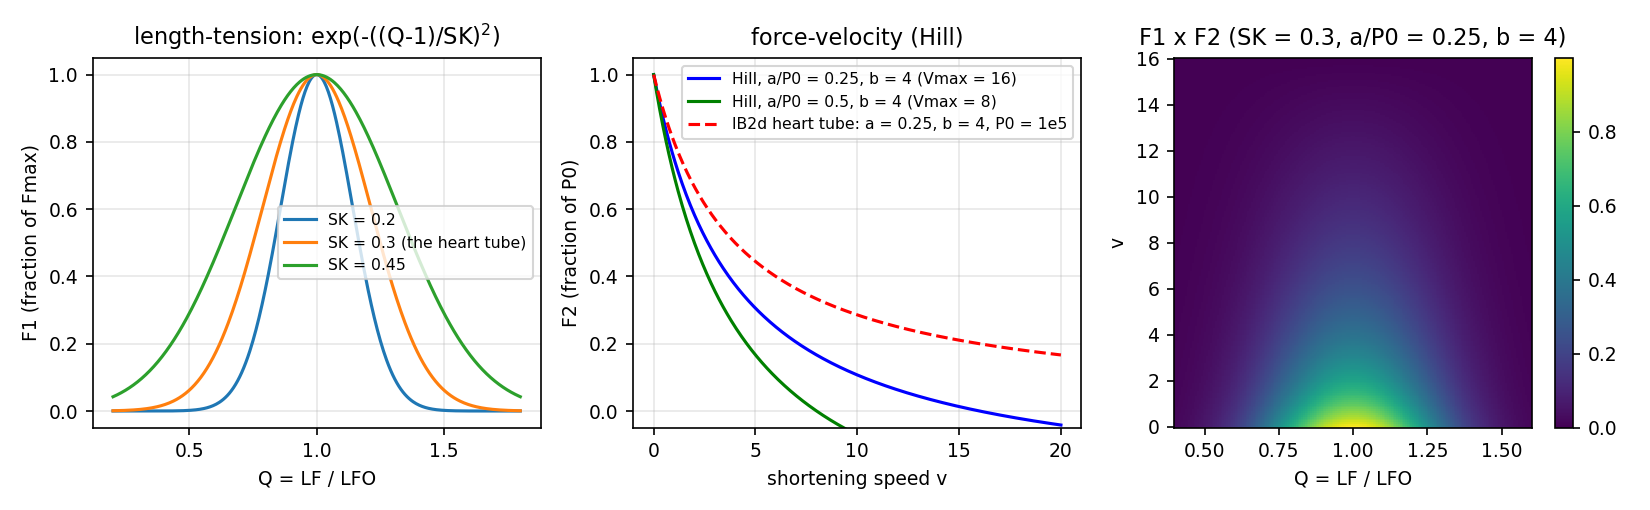
\includegraphics[width=0.9\textwidth]{ch4e-muscle-lt-fv.png}

\raggedright\footnotesize
\al{Length--tension.} The tension a sarcomere can generate depends on its length: at intermediate lengths all myosin heads are within reach of thin filaments; stretched, few overlap; fully contracted, the filaments interfere. (The lecture's figure, unattributed: maximal force for sarcomere lengths of about 1.8--2.2\,$\mu$m, zero near 1.3 and 3.6\,$\mu$m, a knee at about 1.6\,$\mu$m and 80\,\%; Gordon, Huxley and Julian's frog fibres (1966): shoulder at 1.67\,$\mu$m, zero at 3.65\,$\mu$m.) The smooth model IB2d uses:
\[ F_I = F_{IO} \exp\!\Big[-\Big(\frac{Q-1}{SK}\Big)^2\Big], \qquad Q = \frac{L_F}{L_{FO}}, \]
$L_{FO}$ the length of maximal tension, $SK$ a constant for each muscle (the lecture: $SK > 0.28$).
\sourcecredit{The 2015 lecture, slides 6--8; the 2016 talk, pages 62--64; \code{Muscle\_Models/muscle\_curves.py}.}
\end{frame}

\begin{frame}{Force--velocity: Hill's law}
\label{fr:fv}
\small
\al{Force--velocity} (Hill's law for a fully activated, tetanic contraction, a steady-state model):
\[ (P + a)(V + b) = b\,(P_0 + a) \iff V = b\,\frac{P_0 - P}{P + a}, \]
$V$ the shortening speed, $P_0$ the maximal (isometric) load, $V_{\max} = b P_0/a$ the speed with no load; $a$ and $b$ are fitted for each muscle ($a/P_0 \approx 0.25$ in Hill's frog muscle). Normalised:
\[ F_2(V) = \frac{P}{P_0} = \frac{b - (a/P_0)\,V}{V + b}. \]
\sourcecredit{The 2015 lecture, slides 6--8; the 2016 talk, pages 62--64; \code{Muscle\_Models/muscle\_curves.py}.}
\end{frame}

\begin{frame}[fragile]{The combined model, and IB2d's code for it}
\label{fr:fvlt}
\begin{columns}[T]
\column{0.47\textwidth}
\small
Assume the force for a given length and velocity is the product of the normalised laws, scaled by an activation:
\[ F_{\text{muscle}}(L_F, V_F) = a_F\, F_{\max}\, F_1(L_F)\, F_2(V_F), \]
$a_F \in [0, 1]$ the normalised degree of activation, $F_{\max}$ the maximal isometric force, $F_1$ the normalised length--tension law, $F_2$ the normalised Hill law.

``Active force comes from force generated by actin \& myosin crossbridges at [sarcomere] level. It is fully extensible when inactive, but shortens when active!'' (the 2016 talk; the 2015 lecture's slide 12 has the longer form it shortens)
\sourcecredit{The 2015 lecture, slides 9--10; the 2016 talk, pages 60--65.}
\column{0.51\textwidth}
\begin{lstlisting}[style=pytiny]
# .muscle rows: leader follower LFO SK a b Fmax
dx = xLag[id_Follower] - xLag[id_Leader]
dy = yLag[id_Follower] - yLag[id_Leader]
LF = np.sqrt( dx**2 + dy**2 )          # length now
LF_P = np.sqrt( dx_P**2 + dy_P**2 )    # length one step ago
v =  np.abs(LF-LF_P)/dt                # speed
from give_Muscle_Activation import give_Muscle_Activation
Fm = give_Muscle_Activation(v,LF,LFO_Vec,SK_Vec,a_Vec,b_Vec,
                            FMAX_Vec,current_time,xPt,np.array(xLag))
mF_x = Fm*(dx/LF); mF_y = Fm*(dy/LF)
fx[id_Leader] += mF_x; fx[id_Follower] -= mF_x   # (in a loop)

# give_Muscle_Activation.py, in the example's folder:
Q = LF/LFO
F1 = np.exp(-((Q-1)/SK)**2)
F2 = (1/P0)*(b*P0-a*v)/(v+b)           # P0 = Fmax
Fm = af_Val*Fmax*F1*F2                 # af from the activation wave
\end{lstlisting}
\scriptsize \code{give\_Muscle\_Force\_Densities} and the heart tube's activation file, abridged. A positive $F_m$ pulls the two points together.
\end{columns}
\end{frame}

\begin{frame}{Three things the code does that the model does not say}
\label{fr:fvltnotes}
\small
\begin{enumerate}
  \item \al{The speed has no sign.} \code{v = |LF - LF\_P|/dt}: a muscle being stretched is treated as one shortening at the same speed, so its force drops along Hill's curve. Real muscle resists lengthening with \emph{more} than $P_0$ (eccentric contraction); Hill's law is for shortening only. Both ports do this (MATLAB: \code{v = abs(LF-LF\_P)/dt}).
  \item \al{$a$ is in force units.} $F_2 = (bP_0 - a v)/(P_0(v + b))$ with the heart tube's $a = 0.25$, $b = 4$, $P_0 = F_{\max} = 10^5$ is $4/(v + 4)$ to within a relative $6 \cdot 10^{-7}\,v$ (six digits for $v \lesssim 1$, four to five at the run's fastest muscles, $v \approx 85$ between dumps): $V_{\max} = bP_0/a = 1.6 \cdot 10^6$, so the muscle never stalls. If $0.25$ was meant as Hill's $a/P_0$, the file should hold $a = 2.5 \cdot 10^4$ (the red dashed curve against the blue one on slide \ref{fr:ltfv}).
  \item \al{The activation sees only the leader's $x$.} \code{give\_Muscle\_Activation} is called with the leader point's $x$ and the whole \code{xLag}; any dependence on $y$, on the follower, on the muscle's own state (fatigue, calcium) has to be built from those.
\end{enumerate}
\begin{punchbox}
\small None of these is a bug in the sense of a crash; they are modelling choices made in the code and not in the slides. Read the force routine before you trust a parameter's units.
\end{punchbox}
\end{frame}

\begin{frame}{The heart tube with muscles: \code{HeartTube\_Muscle}}
\label{fr:tube}
\begin{columns}[T]
\column{0.5\textwidth}
\footnotesize
\begin{itemize}
  \item A tube of diameter $d = 1$ and length 3 (two rows of 155 points, $x$ from 1 to 4, $y = 2$ and $3$) in a $5 \times 5$ box, $128^2$, $\mu = 0.1$, $\Delta t = 5 \cdot 10^{-4}$, $T = 0.25$.
  \item Springs $k = 10^7$ along each wall, beams $k_b = 7.5 \cdot 10^7$ (straight), one target point at each end of each wall ($k_t = 10^6$): the tube floats.
  \item 153 muscles across the tube, each from a point of one wall to the point opposite: $L_{FO} = d = 1$, $SK = 0.3$, $a = 0.25$, $b = 4$, $F_{\max} = 10^5$.
  \item The activation: a square pulse, width $L_{AR}/10 = 0.15$, that sweeps the middle half of the tube ($1.75 \le x \le 3.25$) left to right at speed $13.5$, once every $0.1$ (\code{freq = 10}), then starts again: 7 or 8 muscles on at a time (right).
\end{itemize}
\column{0.48\textwidth}
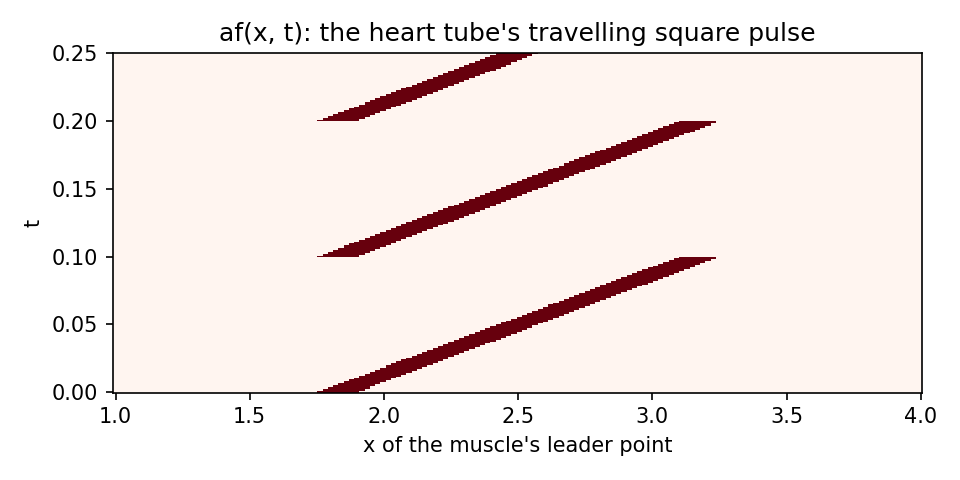
\includegraphics[width=\textwidth]{ch4e-activation-wave.png}
\scriptsize \code{Muscle\_Models/activation\_wave.py}: the example's activation function copied line for line, evaluated on the example's points without the fluid (what its \code{test\_Activation\_Wave.py} does).
\end{columns}
\end{frame}

\begin{frame}{The heart tube, run}
\label{fr:tuberun}
\centering
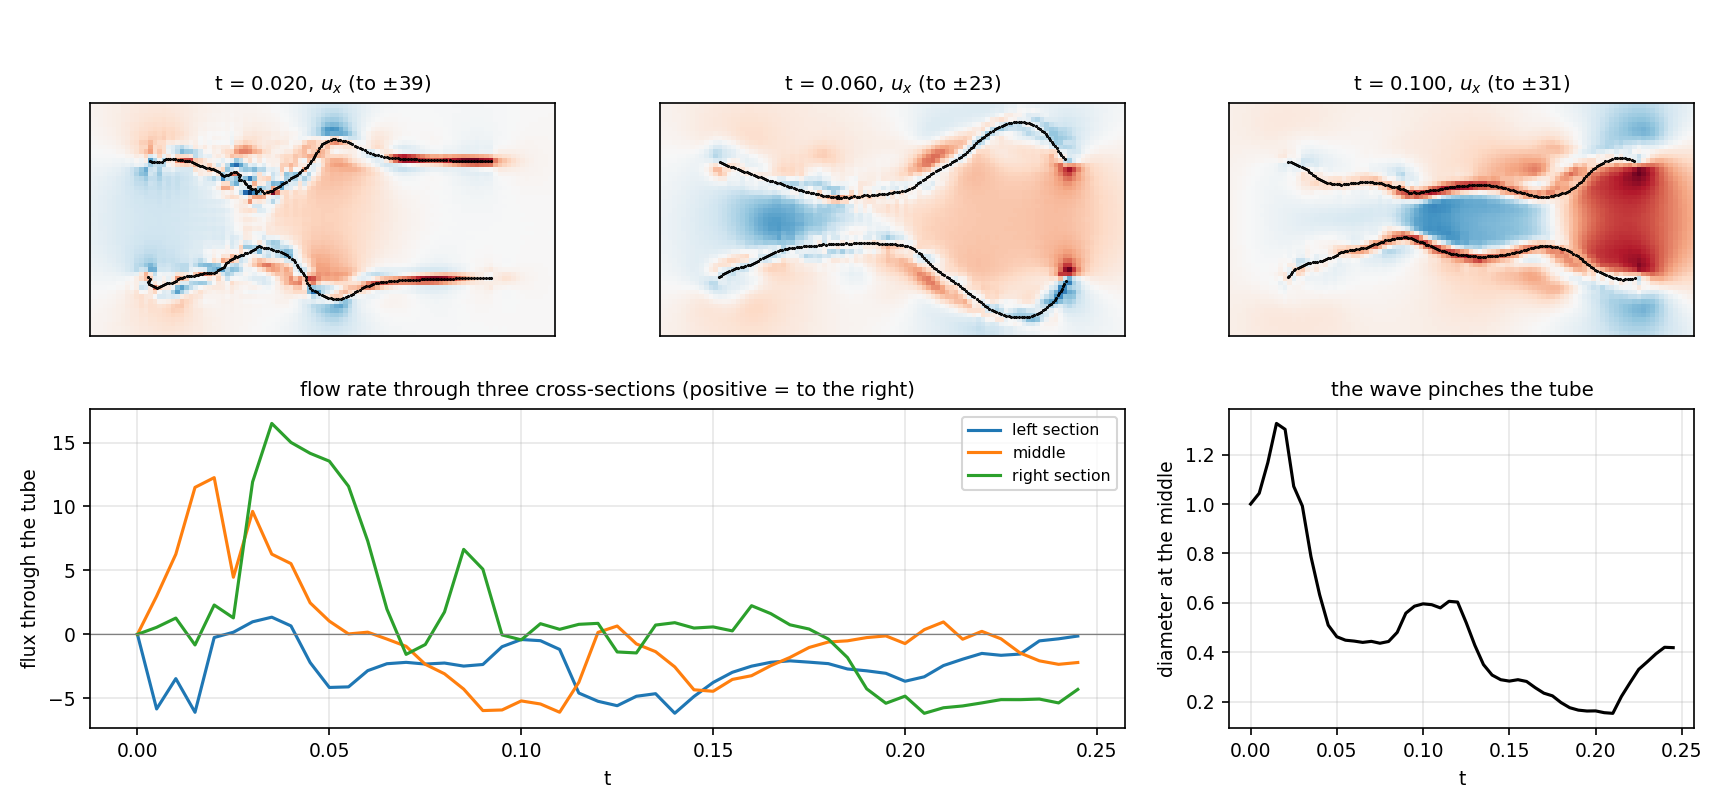
\includegraphics[width=0.88\textwidth]{ch4e-hearttube.png}

\scriptsize
Top: $u_x$ (red to the right, blue to the left) at $t = 0.02$, $0.06$, $0.10$, each frame on its own scale. Bottom left: the flow rate $\int u_x\,dy$ across the tube at $x = 1.75$, $2.5$ and $3.25$. Bottom right: the tube's diameter at $x = 2.5$. 500 steps, 9.5 s.
\end{frame}

\begin{frame}{Reading the heart tube}
\label{fr:tuberead}
\footnotesize
\begin{itemize}
  \item \al{The pinch is strong:} the diameter at the middle ($x = 2.5$) first bulges to 1.33 ($t = 0.015$, before the first pulse arrives), falls to 0.46 as that pulse passes ($t \approx 0.05$) and keeps falling, to 0.15 at $t = 0.21$ (the third pulse is then still upstream), before it reopens to 0.42: the wall lags the activation. With only four target points the whole tube flexes and its ends flail. The first frames carry a start-up transient on the walls (chapter 4b saw the same).
  \item \al{The flow oscillates} with every pulse (rates from $-6.2$ to $+16.5$), and its mean over the last full period ($0.15 \le t < 0.25$) is negative at all three sections: $-2.2$, $-1.3$ and $-2.9$; over the first period ($0 \le t < 0.1$) it was $-2.0$, $+2.0$ and $+5.4$. In this run the tube moved fluid \emph{to the left}, against the activation wave, only after its first period; which way it pumps once it is periodic is open. The three means differ by more than the noise: in 2.5 periods the tube's volume has not settled into a periodic state.
  \item The talk shows this example with the warning ``PARAMETERS ARE NOT FINELY TUNED!!!!!''. A pumping study starts here: longer runs (many periods), walls held better, the flux over whole periods at several sections until they agree, then the parameters (pulse speed, width, $F_{\max}$, the $a$ of slide \ref{fr:fvltnotes}).
\end{itemize}
\begin{punchbox}
\small Measure what a pump does over whole periods and at more than one section before you say which way it pumps. Valveless pumps can pump either way, and their net flow is highly sensitive to the pinching frequency (impedance pumping: Hickerson, Rinderknecht and Gharib 2005; chapter 4b's tracer pump is one).
\end{punchbox}
\end{frame}

% ---------------------------------------------------------------- three-element Hill
\begin{frame}{The three-element Hill model}
\label{fr:hill3}
\begin{columns}[T]
\column{0.3\textwidth}
\centering
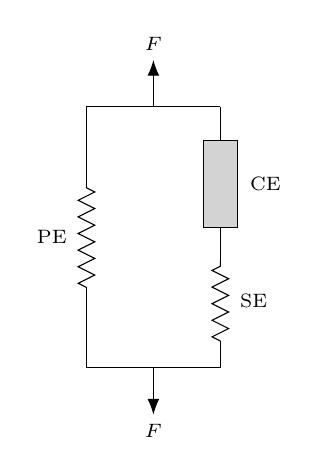
\begin{tikzpicture}[scale=0.85]
  \draw[-{Latex[length=2mm]}] (1,4.2) -- (1,4.9) node[above,font=\scriptsize] {$F$};
  \draw[-{Latex[length=2mm]}] (1,0.3) -- (1,-0.4) node[below,font=\scriptsize] {$F$};
  \draw (0,0.3) -- (2,0.3); \draw (0,4.2) -- (2,4.2);
  \draw (0,0.3) -- (0,1.5); \draw[decorate,decoration={zigzag,amplitude=3pt,segment length=6pt}] (0,1.5) -- (0,3.0); \draw (0,3.0) -- (0,4.2);
  \node[font=\scriptsize,left] at (-0.15,2.25) {PE};
  \draw (2,0.3) -- (2,0.7); \draw[decorate,decoration={zigzag,amplitude=3pt,segment length=6pt}] (2,0.7) -- (2,1.9); \draw (2,1.9) -- (2,2.4);
  \node[font=\scriptsize,right] at (2.15,1.3) {SE};
  \draw[fill=LightGray] (1.75,2.4) rectangle (2.25,3.7); \draw (2,3.7) -- (2,4.2);
  \node[font=\scriptsize,right] at (2.3,3.05) {CE};
\end{tikzpicture}
\column{0.68\textwidth}
\footnotesize
A contractile element (CE) in series with an elastic element (SE), the pair in parallel with another elastic element (PE).
\begin{itemize}
  \item \al{CE}: the active force of the actin--myosin crossbridges; fully extensible when inactive, able to shorten when activated. Use the combined law: $F_{CE} = a_F F_{\max} F_1(L_{CE}) F_2(V_{CE})$.
  \item \al{PE}: the passive connective tissue; resists stretch even when the CE is off.
  \item \al{SE}: the tendon and the filaments' own elasticity; stores energy.
\end{itemize}
Forces and lengths:
\[ F = F_{PE} + F_{SE}, \quad F_{CE} = F_{SE}; \qquad L = L_{PE}, \quad L = L_{CE} + L_{SE}; \]
with nonlinear springs, e.g.\ $F_{SE} = F_{CE} = k_{SE}(L - L_{CE})^3$ (zero resting length) and $F_{PE} = k_{PE}(L - L_R)^3$ (resting length $L_R$). ``There are many other ways to model each elastic element, and these will depend upon the animal considered.''
\end{columns}
\sourcecredit{The 2015 lecture, slides 11--16. The series element and the CE carry the same force: given $L$, solve $F_{CE}(L_{CE}, \dot L_{CE}) = k_{SE}(L - L_{CE})^3$ for $L_{CE}$ every step.}
\end{frame}

\begin{frame}{What IB2d's three-element code computes (MATLAB)}
\label{fr:hill3code}
\footnotesize
\code{IBM\_Driver.m}'s \code{read\_Hill\_3Muscle\_Points} reads nine columns per muscle from \code{<name>.3\_muscle} (lines 2057--2072), and \code{give\_3\_Element\_Muscle\_Force\_Densities} uses them: \code{leader follower LFO SK a b Fmax kSpr alpha}. For each muscle, with $d = \mathbf{X}_f - \mathbf{X}_l$, $L_F = |d|$ and $v = |L_F - L_F^{\text{prev}}|/\Delta t$, the example's activation file returns $F_m$ (the combined law), a switch \code{on\_Parallel}, a coefficient \code{PE\_Coeff} and the activation $a_f$, and the leader receives
\[ \underbrace{F_m\,\frac{d}{L_F}}_{\text{CE}} \;\underbrace{-\, a_f\,k_{\text{Spr}}\,d \,+\, 1.0\cdot\dot{\mathbf{X}}_l}_{\text{``SE''}} \;+\; \underbrace{\text{PE\_Coeff}\cdot\tfrac12(\alpha + 1)\,k_{\text{Spr}}\,(L_F - L_{FO})^{\alpha}\,\frac{d}{L_F}}_{\text{PE, if on\_Parallel}}, \]
the follower the opposite (lines 671--753; the ``SE'' term is coded as $a_f k_{\text{Spr}}((L_{FO} - L_F) - L_{FO})\,d/L_F$, with the comment ``L\_con (LF) + L\_ser = L\_tot = LFO'').
\begin{itemize}
  \item The CE and SE forces are \al{added}, not set equal; there is no separate $L_{CE}$, so it is not the series arrangement of the previous slide.
  \item The ``SE'' part is $-a_f k_{\text{Spr}}\,d$ on the leader: it pushes the two points \emph{apart}, in proportion to their distance, while active.
  \item The damping term adds $1.0 \times$ the leader's velocity to the leader's force: a force \emph{along} the motion, the opposite sign of a damper, and it acts whether or not the muscle is active.
\end{itemize}
\sourcecredit{\code{matIB2d/IBM\_Blackbox/please\_Find\_Lagrangian\_Forces\_On\_Eulerian\_grid.m}, read, not run (Octave cannot run matIB2d).}
\end{frame}

\begin{frame}[fragile]{The three-element model in practice: which examples match the code}
\label{fr:hill3state}
\small
\begin{itemize}
  \item \al{MATLAB.} The black box calls \code{[Fm,on\_Parallel,PE\_Coeff,af\_Val] =}\allowbreak\code{ give\_3\_Element\_Muscle\_Activation(}\allowbreak\code{v,LF,LFO,sk,a,b,Fmax,}\allowbreak\code{current\_time,xPt,xLag,i)}: eleven inputs, four outputs. Of the three examples that use the model, only \code{Example\_Scallop/Scallop\_3Elem\_Muscle} has a matching activation file (and the \code{.3\_muscle} file). \code{Scallop\_3Elem\_Muscle\_Almost\_Swims} defines ten inputs and three outputs; \code{Example\_HeartTube/3\_Element\_Muscle\_Model} defines ten inputs and one output, and has no \code{HeartTube.3\_muscle}. By their signatures, those two do not run with the 2024 black box.
  \item \al{Python.} The README (\code{pyIB2d/README.txt}) marks the model ``UNTESTED!! THIS IS LIKELY BROKEN.'' It is: the reader takes seven columns from \code{.muscle} (no \code{kSpr}, \code{alpha}), the force routine has no SE or PE terms, and it calls a function it never imports. The heart tube with \code{FV\_LT\_muscle = 0} and \code{3\_element\_muscle = 1} stops at the first step:
\end{itemize}
\vspace{-1mm}
\begin{lstlisting}[style=tiny]
  File ".../please_Find_Lagrangian_Forces_On_Eulerian_grid.py", line 465,
    in give_3_Element_Muscle_Force_Densities
    Fm = give_3_Element_Muscle_Activation(v,LF,LFO_Vec,SK_Vec,a_Vec,b_Vec,\
NameError: name 'give_3_Element_Muscle_Activation' is not defined. Did you mean: 'give_3_Element_Muscle_Force_Densities'?
\end{lstlisting}
\vspace{-1mm}
\small For a three-element muscle in IB2d today: MATLAB and the scallop's files, read with the previous slide in mind; or write it as a user-defined force (slide \ref{fr:user}), with the series element solved properly.
\end{frame}

% ---------------------------------------------------------------- crossbridges
\begin{frame}{Part 3: crossbridges}
\label{fr:xb}
\begin{columns}[T]
\column{0.4\textwidth}
\resizebox{\linewidth}{!}{%
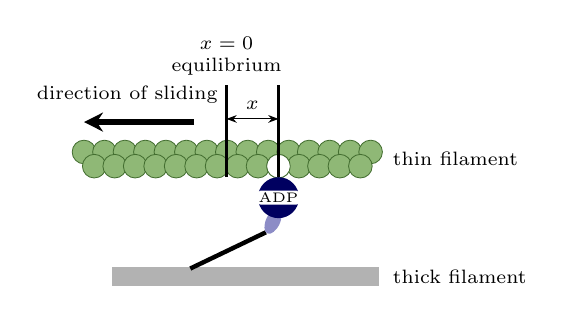
\begin{tikzpicture}[font=\scriptsize]
  % the thick filament
  \fill[gray!60] (0.9,-0.40) rectangle (4.3,-0.16);
  \node[anchor=west] at (4.35,-0.28) {thick filament};
  % the thin filament: two staggered rows of actin beads; the site the head holds is white
  \foreach \i in {0,...,14} {\fill[OliveGreen!50, draw=OliveGreen!80!black, line width=0.3pt] ({0.55+0.26*\i},1.30) circle (0.15);}
  \foreach \i in {0,...,13} {\fill[OliveGreen!50, draw=OliveGreen!80!black, line width=0.3pt] ({0.68+0.26*\i},1.12) circle (0.15);}
  \fill[white, draw=OliveGreen!80!black, line width=0.3pt] (3.02,1.12) circle (0.15);
  \node[anchor=west] at (4.35,1.21) {thin filament};
  % the crossbridge: neck from the thick filament, lever, head (holding ADP) on the thin filament
  \draw[line width=1.6pt] (1.9,-0.18) -- (2.86,0.28);
  \fill[NavyBlue!45, rotate around={-25:(2.95,0.42)}] (2.95,0.42) ellipse [x radius=0.09, y radius=0.17];
  \fill[NavyBlue!75!black] (3.02,0.72) circle (0.26);
  \node[fill=white, rounded corners=1.5pt, inner sep=0.8pt, font=\fontsize{4.5}{4.5}\selectfont] at (3.02,0.72) {ADP};
  % x: the site's displacement from the equilibrium configuration
  \draw[line width=0.9pt] (2.36,0.98) -- (2.36,2.15);
  \draw[line width=0.9pt] (3.02,0.98) -- (3.02,2.15);
  \draw[{Stealth[length=1.3mm]}-{Stealth[length=1.3mm]}] (2.36,1.72) -- (3.02,1.72) node[midway,above] {$x$};
  \node[anchor=south, align=center] at (2.36,2.15) {$x = 0$\\equilibrium};
  % the thin filament slides to the left
  \draw[-{Stealth[length=2.4mm,width=2.4mm]}, line width=2pt] (1.95,1.68) -- (0.55,1.68);
  \node[anchor=south] at (1.1,1.8) {direction of sliding};
\end{tikzpicture}}

\vspace{2mm}
\resizebox{\linewidth}{!}{%
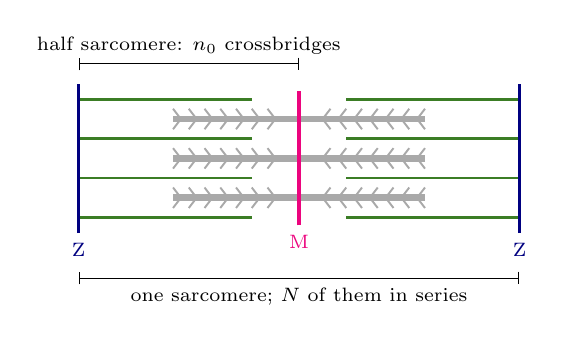
\begin{tikzpicture}[font=\scriptsize]
  % thin filaments from the Z lines; thick filaments with heads, bare in the middle
  \foreach \y in {0.15,0.65,1.15,1.65} {\draw[line width=1pt,OliveGreen] (0,\y) -- (2.2,\y); \draw[line width=1pt,OliveGreen] (3.4,\y) -- (5.6,\y);}
  \foreach \y in {0.4,0.9,1.4} {
    \draw[line width=2.4pt,DarkGray] (1.2,\y) -- (4.4,\y);
    \foreach \x in {1.3,1.5,...,2.5} {\draw[DarkGray,line width=0.7pt] (\x,\y) -- ++(-0.1,0.13); \draw[DarkGray,line width=0.7pt] (\x,\y) -- ++(-0.1,-0.13);}
    \foreach \x in {3.1,3.3,...,4.3} {\draw[DarkGray,line width=0.7pt] (\x,\y) -- ++(0.1,0.13); \draw[DarkGray,line width=0.7pt] (\x,\y) -- ++(0.1,-0.13);}
  }
  \draw[very thick,NavyBlue] (0,-0.05) -- (0,1.85); \draw[very thick,NavyBlue] (5.6,-0.05) -- (5.6,1.85);
  \draw[very thick,RubineRed] (2.8,0.05) -- (2.8,1.75);
  \node[NavyBlue,below] at (0,-0.05) {Z}; \node[NavyBlue,below] at (5.6,-0.05) {Z}; \node[RubineRed,below] at (2.8,0.05) {M};
  \draw[|-|] (0,2.1) -- (2.8,2.1) node[midway,above] {half sarcomere: $n_0$ crossbridges};
  \draw[|-|] (0,-0.62) -- (5.6,-0.62) node[midway,below] {one sarcomere; $N$ of them in series};
\end{tikzpicture}}
\column{0.58\textwidth}
\footnotesize
\begin{itemize}
  \item \al{Equilibrium configuration}: where the crossbridge exerts no force on the thin filament; $x$ is the distance from it.
  \item $p(x)$: the force on the thin filament when the crossbridge is displaced by $x$; $p(0) = 0$.
  \item $n_0$: the number of crossbridges in a half sarcomere; they act in parallel (forces add): all attached and displaced by $x$ give $n_0\,p(x)$.
  \item $N$: the number of sarcomeres; the $2N$ half sarcomeres are in series (lengths add).
  \item $u(x)$: the population density of attached crossbridges. The fraction attached between $x_1$ and $x_2$ is $\int_{x_1}^{x_2} u\,dx$; the total fraction attached is $U = \int_{-\infty}^{\infty} u\,dx$; and the force on the ends of the muscle is
  \[ P = n_0 \int_{-\infty}^{\infty} p(x)\,u(x)\,dx. \]
\end{itemize}
\end{columns}
\sourcecredit{The 2015 lecture, slides 19--22; the crossbridge (its slide 20) and the sarcomere (its slide 21) redrawn here.}
\end{frame}

\begin{frame}{Attach, slide, detach}
\label{fr:xb2}
\begin{columns}[T]
\column{0.4\textwidth}
\resizebox{\linewidth}{!}{%
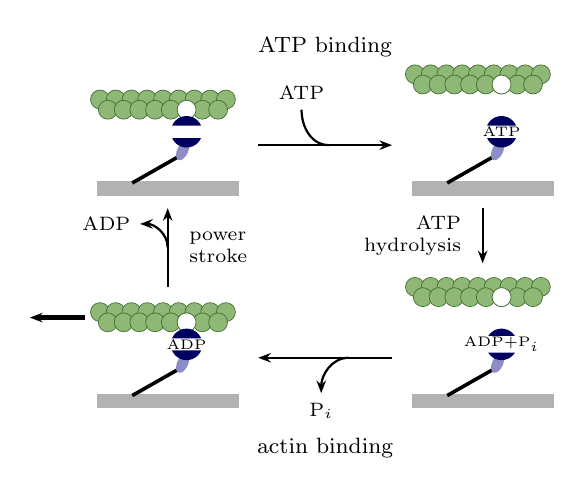
\begin{tikzpicture}[font=\scriptsize, >={Stealth[length=1.6mm]}]
  \xbstate{0}{2.7}{0}{\phantom{ATP}}
  \xbstate{4}{2.7}{0.32}{ATP}
  \xbstate{4}{0}{0.32}{ADP+P$_i$}
  \xbstate{0}{0}{0}{ADP}
  % ATP binds: the head lets go
  \draw[->, thick] (1.15,3.25) -- (2.85,3.25);
  \draw[thick] (1.7,3.7) to[out=-90,in=180] (2.05,3.25);
  \node[above] at (1.7,3.7) {ATP};
  \node[font=\footnotesize] at (2.0,4.5) {ATP binding};
  % hydrolysis: the head is cocked
  \draw[->, thick] (4,2.45) -- (4,1.75);
  \node[anchor=east, align=right] at (3.85,2.1) {ATP\\hydrolysis};
  % the head binds actin and releases P_i
  \draw[->, thick] (2.85,0.55) -- (1.15,0.55);
  \draw[->, thick] (2.3,0.55) to[out=180,in=90] (1.95,0.1);
  \node[below] at (1.95,0.1) {P$_i$};
  \node[font=\footnotesize] at (2.0,-0.6) {actin binding};
  % the power stroke releases ADP; the thin filament slides
  \draw[->, thick] (0,1.45) -- (0,2.45);
  \draw[->, thick] (0,1.95) to[out=90,in=0] (-0.35,2.25);
  \node[left] at (-0.35,2.25) {ADP};
  \node[anchor=west, align=left] at (0.15,1.95) {power\\stroke};
  \draw[->, line width=1.6pt] (-1.05,1.06) -- (-1.75,1.06);
\end{tikzpicture}}
\sourcecredit{The 2015 lecture, slide 18 (redrawn): the ATPase--crossbridge cycle after Lymn and Taylor (1971).}
\column{0.58\textwidth}
\footnotesize
\begin{itemize}
  \item \al{Attach}: crossbridges attach at $x = A > 0$, at a rate proportional to the number available, $n_0(1 - U)$: rate $\alpha\,n_0(1 - U)$.
  \item \al{Slide}: attached crossbridges move with the filament, $dx/dt = -v$, $v$ the shortening speed of the thin filament relative to the thick one; for the whole muscle $V = 2Nv$.
  \item \al{Detach}: at a rate $\beta$ per attached crossbridge, independent of $x$: from $(x_1, x_2)$ at rate $\beta n_0 \int_{x_1}^{x_2} u\,dx$; in total $\beta n_0 U$.
\end{itemize}
In steady shortening, crossbridges with $x_0 < x < A$ are replenished by attachment and lost by detachment and by sliding past $x_0$ (rate $v\,n_0\,u(x_0)$). Balance:
\[ \alpha\,(1 - U) = \beta \int_{x_0}^{A} u(x)\,dx + v\,u(x_0). \]
\end{columns}
\end{frame}

\begin{frame}{The steady state}
\label{fr:xb3}
\small
The balance holds for every $x_0 < A$. Differentiate with respect to $x_0$:
\[ 0 = -\beta\,u(x_0) + v\,\frac{du}{dx_0} \quad\Longrightarrow\quad v\,\frac{du}{dx} = \beta u, \qquad u(x) = u(A)\,\exp\!\Big(\frac{\beta(x - A)}{v}\Big) \ \ (x < A), \]
and $u(x) = 0$ for $x > A$ (nothing attaches there). Two conditions fix $u(A)$ and $U$:
\[ x_0 = A: \ \ \alpha(1 - U) = v\,u(A); \qquad U = \int_{-\infty}^{A} u(A)\,e^{\beta(x - A)/v}\,dx = \frac{v\,u(A)}{\beta}; \]
so
\[ U = \frac{\alpha}{\alpha + \beta}, \qquad u(A) = \frac{\alpha\beta}{v\,(\alpha + \beta)}, \qquad u(x) = \frac{\alpha\beta}{v\,(\alpha + \beta)}\,\exp\!\Big(\frac{\beta(x - A)}{v}\Big). \]
The fraction attached does not depend on the speed; how far the attached bridges are dragged before they let go does: the faster the shortening, the more bridges sit at $x < 0$ pulling backwards.
\sourcecredit{The 2015 lecture, slides 28--32, which give no source for this form: Huxley's (1957) crossbridge model, simplified to attachment at one point and detachment at a constant rate.}
\end{frame}

\begin{frame}{Hill's law from crossbridges}
\label{fr:xb4}
\begin{columns}[T]
\column{0.52\textwidth}
\scriptsize
With the nonlinear crossbridge spring $p(x) = p_1(e^{\gamma x} - 1)$ (a linear $p = kx$ gives a linear force--velocity curve),
\[ P = \frac{\alpha\beta}{v(\alpha+\beta)} \int_{-\infty}^{A} n_0 p(x)\, e^{\beta(x - A)/v}\,dx \]
\[ \phantom{P} = K\,\frac{(e^{\gamma A} - 1) - \gamma v/\beta}{1 + \gamma v/\beta}, \]
$K = \alpha n_0 p_1/(\alpha + \beta)$. Solve for $\gamma v/\beta$ and use $V = 2Nv$:
\[ V = b\,\frac{P_0 - P}{P + a}, \quad a = K, \quad b = \frac{2N\beta}{\gamma}, \quad P_0 = K(e^{\gamma A} - 1), \]
\[ V_{\max} = \frac{2N\beta}{\gamma}\,(e^{\gamma A} - 1), \quad \frac{a}{P_0} = \frac{1}{e^{\gamma A} - 1}. \]
``Using this analysis, we have derived the empirical force--velocity curve from a model of crossbridge dynamics.'' Hill's $a/P_0 \approx 0.25$ means $\gamma A = \ln 5$.
\column{0.46\textwidth}
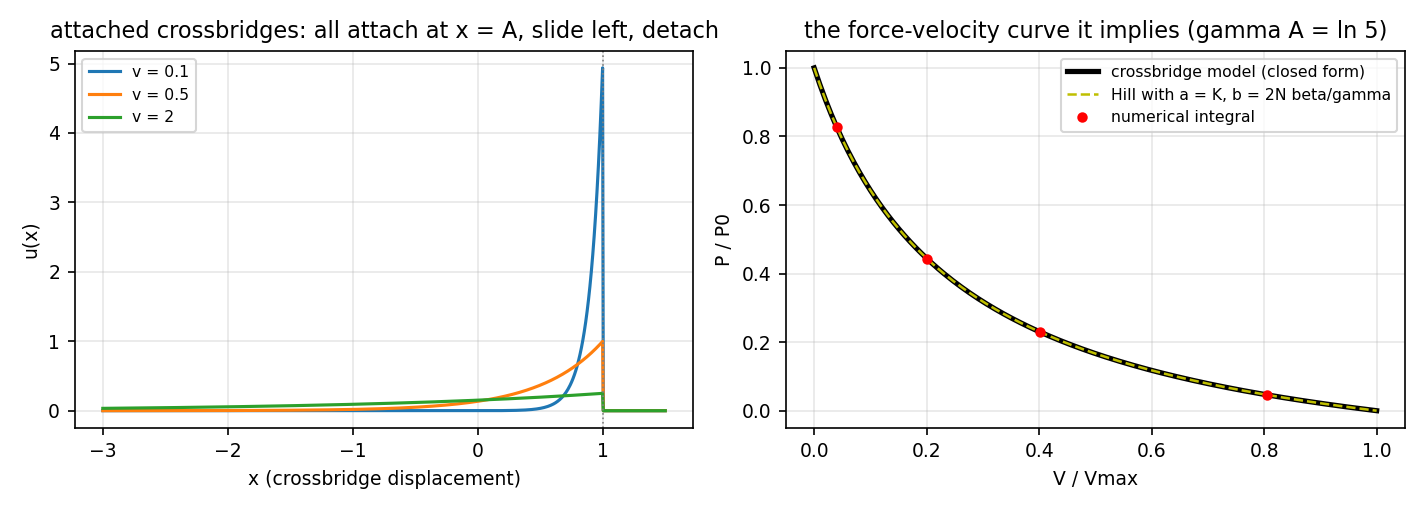
\includegraphics[width=\textwidth]{ch4e-muscle-huxley.png}
\scriptsize \code{Muscle\_Models/muscle\_curves.py} with $\alpha = \beta = A = n_0 p_1 = N = 1$, $\gamma = \ln 5$: left, $u(x)$ at three speeds; right, the closed form (black), Hill's law with the derived $a$, $b$ (yellow dashes) and the integral $n_0\int p\,u\,dx$ computed numerically (red dots, four of the six speeds checked). The closed form and the numerical integral agree to $5 \cdot 10^{-8}$ of $P_0$ at six speeds.
\end{columns}
\sourcecredit{The 2015 lecture, slides 33--38.}
\end{frame}

% ---------------------------------------------------------------- activation
\begin{frame}{Part 4: activation, from nerve to crossbridge}
\label{fr:act}
\centering
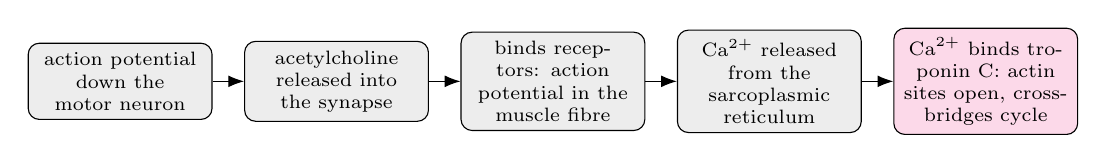
\begin{tikzpicture}[node distance=3mm and 4mm, every node/.style={font=\scriptsize, align=center}]
  \node[draw,rounded corners,fill=LightGray!40,text width=2.1cm] (a) {action potential down the motor neuron};
  \node[draw,rounded corners,fill=LightGray!40,text width=2.1cm,right=of a] (b) {acetylcholine released into the synapse};
  \node[draw,rounded corners,fill=LightGray!40,text width=2.1cm,right=of b] (c) {binds receptors: action potential in the muscle fibre};
  \node[draw,rounded corners,fill=LightGray!40,text width=2.1cm,right=of c] (d) {Ca$^{2+}$ released from the sarcoplasmic reticulum};
  \node[draw,rounded corners,fill=RubineRed!15,text width=2.1cm,right=of d] (e) {Ca$^{2+}$ binds troponin C: actin sites open, crossbridges cycle};
  \foreach \u/\v in {a/b,b/c,c/d,d/e} {\draw[-{Latex[length=2mm]}] (\u) -- (\v);}
\end{tikzpicture}

\vspace{3mm}
\small
\begin{itemize}
  \item If enough acetylcholine binds, an action potential is induced in the muscle fibre; it releases calcium ions from the sarcoplasmic reticulum into the cell.
  \item Contraction happens when calcium bound to troponin opens the myosin-binding sites on actin, so crossbridges can form and cycle, producing force.
  \item \al{End of contraction}: acetylcholinesterase in the synapse breaks acetylcholine down within milliseconds; with no acetylcholine on the receptors, calcium is taken back into the sarcoplasmic reticulum and the binding sites close.
\end{itemize}
\sourcecredit{The activation tutorial, slides 2--7 (its textbook figures are described here, not copied).}
\end{frame}

\begin{frame}{Varying the force: summation, fibre types, tetanus}
\label{fr:summation}
\small
Nerve impulses are, for the most part, all alike; muscles still produce graded forces, by \al{force summation}:
\begin{itemize}
  \item \al{Multiple fibre summation}: a weak signal recruits the small, more excitable motor units first; stronger signals add more and larger units (the largest up to about 50 times stronger than the smallest).
  \item \al{Frequency summation}: action potentials arriving faster; twitches add before the previous one has relaxed. At high enough frequency the muscle does not relax between stimuli: a \al{tetanic} (fused) contraction. During a maximal voluntary effort only about a third of a human muscle's fibres fire at once, which protects the tendon.
\end{itemize}
\al{Fibre types.} A muscle mixes fibre types in proportions that vary within and across species and with training. Slow-twitch fibres contract more slowly and fatigue late; fast-twitch fibres release calcium faster, split ATP faster and fatigue sooner. Chicken legs (walking, standing: dark meat) are mostly slow-twitch; breast and wings (short bursts of flight: white meat) mostly fast-twitch.
\sourcecredit{The activation tutorial, slides 8--14 (the summation text is quoted there from Wikipedia, the chicken example from a BBC Science page).}
\end{frame}

\begin{frame}{A calcium model of activation}
\label{fr:calcium}
\begin{columns}[T]
\column{0.5\textwidth}
\footnotesize
Williams et al.'s model for lamprey muscle: the stimulus from the motor neurons is \al{on or off}; the action potential, acetylcholine and depolarisation are not modelled. Mass-action kinetics move calcium between the sarcoplasmic reticulum (bound: $[cs]$, free sites $[s]$), the cytosol ($[c]$) and the thin filaments (bound $[cf]$, free $[f]$): stimulus on, release at rate $k_1[cs]$; off, uptake at $k_2[c][s]$; binding to filaments $k_3[c][f]$, unbinding $k_4[cf][f]$.

Conservation: $[cs] + [c] + [cf] = C_T$, $[cs] + [s] = S_T$, $[cf] + [f] = F_T$. Scale by the filament sites, $Ca = [c]/F_T$, $Caf = [cf]/F_T$, $C = C_T/F_T$, $S = S_T/F_T$ (so $Caf \le 1$).
\column{0.48\textwidth}
\footnotesize
Stimulus \al{on}:
\[ \frac{dCa}{dt} = (k_4 Caf - k_3 Ca)(1 - Caf) \]
\[ \qquad\quad +\, k_1(C - Ca - Caf), \]
stimulus \al{off}:
\[ \frac{dCa}{dt} = (k_4 Caf - k_3 Ca)(1 - Caf) \]
\[ \qquad\quad +\, k_2\,Ca\,(C - S - Ca - Caf), \]
and always
\[ \frac{dCaf}{dt} = -(k_4 Caf - k_3 Ca)(1 - Caf). \]
$Caf$, the fraction of filament sites with calcium bound, is the activation: it multiplies the contractile force (slide \ref{fr:twoel}). The rate constants absorb the factors of $F_T$ from the scaling.
\end{columns}
\sourcecredit{The activation tutorial, slides 15--20.}
\end{frame}

\begin{frame}{Twitches, summation and tetanus from the calcium model}
\label{fr:calciumrun}
\centering
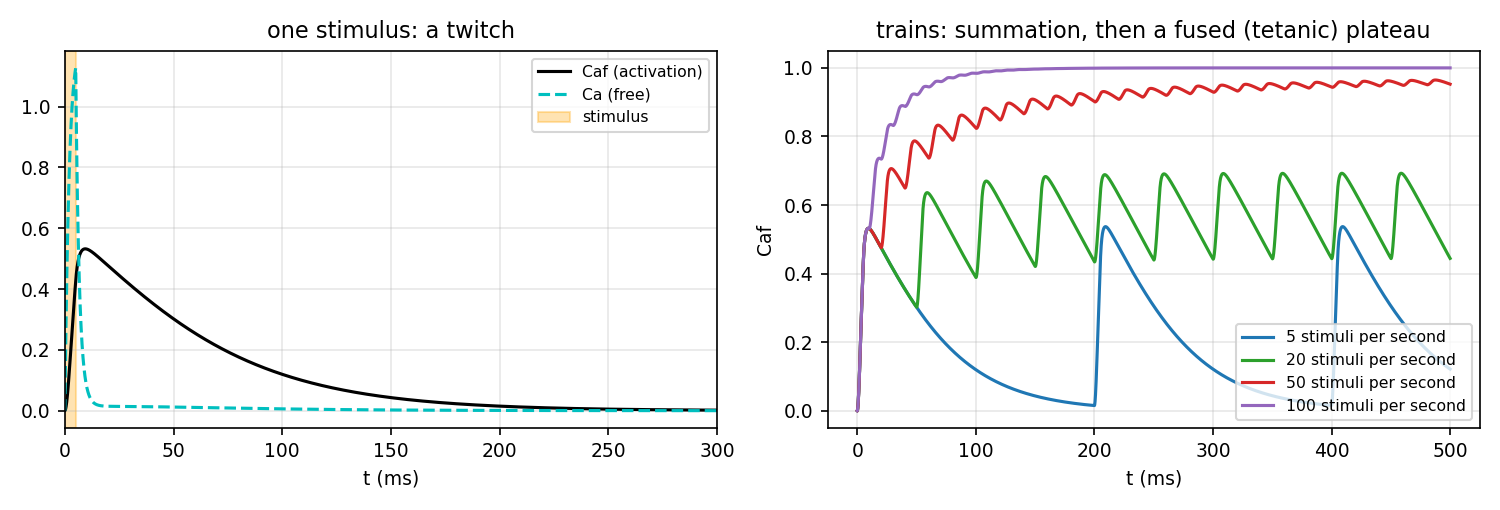
\includegraphics[width=0.86\textwidth]{ch4e-calcium.png}

\footnotesize
\begin{columns}[T]
\column{0.5\textwidth}
\code{Muscle\_Models/calcium\_activation.py} (fixed-step RK4, $\Delta t = 10^{-5}$ s), with \al{illustrative} constants, not fitted values: $k_1 = 300$, $k_2 = 100$, $k_3 = 150$, $k_4 = 30$ per second, $C = 2$, $S = 6$, stimuli of 5 ms.
\column{0.48\textwidth}
One stimulus: $Caf$ peaks at 0.53 after 9 ms and halves at about 57 ms. Trains: at 5 per second the twitches stay separate (0.02--0.54 over the last 0.1 s), at 20 they sum (0.44--0.69), at 50 they fuse into a plateau (0.94--0.96), at 100 the filaments saturate ($Caf = 1.00$).
\end{columns}
\end{frame}

\begin{frame}{IB2d's own calcium model}
\label{fr:calciumib2d}
\begin{columns}[T]
\column{0.5\textwidth}
\scriptsize
The MATLAB heart tubes with calcium (\code{Example\_HeartTube/}: \code{Electromechanical\_Pumping\_w\_Ca\_Dynamics}, its \code{128x128\_} version and \code{EM\_Pump\_w\_Calcium\_and\_Muscles}; slide \ref{fr:map}) solve this model in advance (\code{Calcium\_Dynamics.m}, the same constants in every copy) and feed $0.5\,Caf(t)$ as the stimulus current of a FitzHugh--Nagumo cable between 25 and 30\,\% of its length:
\[ \begin{aligned} \frac{dCa}{dt} &= k_4 Caf - k_3 Ca(1 - Caf) \\ &\quad + k_2\,Ca\,(C - S - Ca - Caf) \\ &\quad \big[ {+}\, k_1 (C - Ca - Caf) \big], \\ \frac{dCaf}{dt} &= -k_4 Caf + k_3 Ca (1 - Caf), \end{aligned} \]
the bracket only during a stimulus. Against slide \ref{fr:calcium}: uptake never stops, and unbinding is $k_4\,Caf$, not $k_4\,Caf\,(1 - Caf)$ (the file: ``removed weird non-biological term''). Forward Euler with $\Delta t = 10^{-5}$\,s; $k_1 = 9$, $k_2 = 50$, $k_3 = 40$, $k_4 = 19.4$ per second, $C = S = 200$; a 5\,ms stimulus every 0.5\,s for the run's 4\,s.
\column{0.48\textwidth}
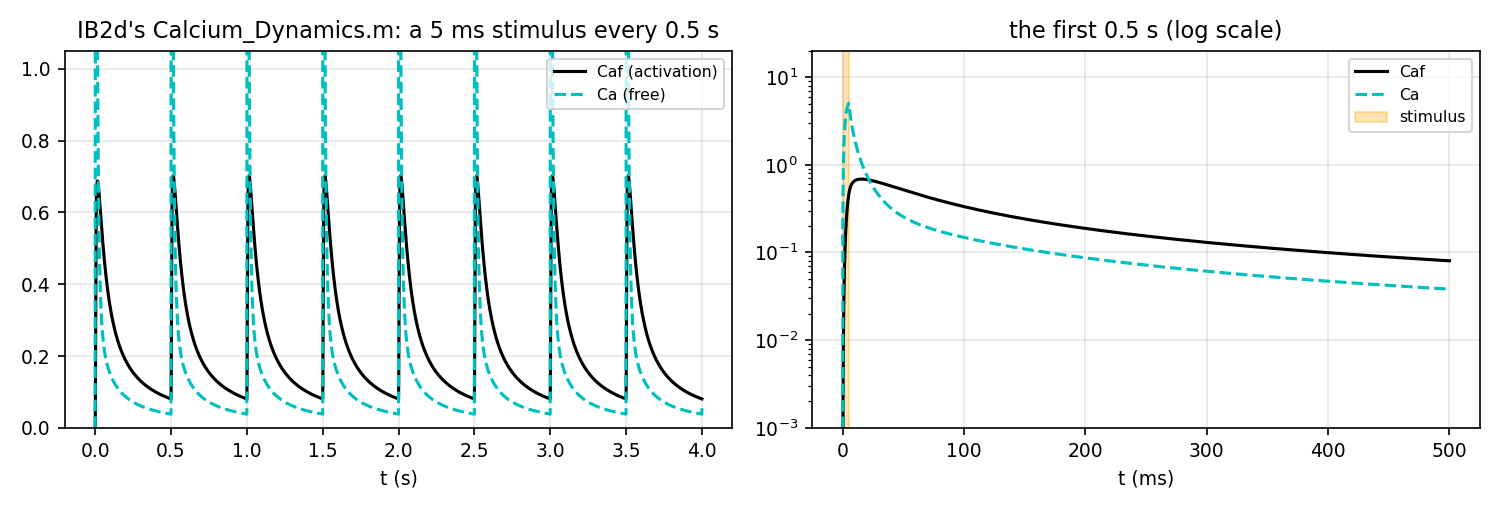
\includegraphics[width=\textwidth]{ch4e-calcium-ib2d.png}

\scriptsize \code{calcium\_activation.py --ib2d}, the file line for line (left, the free calcium is clipped): each stimulus lifts the free calcium to 5.0; $Caf$ peaks at 0.69 (0.70 from the second stimulus on, 2\,\% higher) 15\,ms after the stimulus starts, halves by 96\,ms and is still 0.08 when the next one comes: separate twitches. The \code{128x128\_} copy still ends with its test plot and \code{pause()}, so in MATLAB that example stops at the plot until a key is pressed.
\end{columns}
\sourcecredit{IB2d: \code{matIB2d/Examples/Example\_HeartTube/*/Calcium\_Dynamics.m} and \code{FitzHugh\_Nagumo\_1d.m} (N.\,A. Battista, 2016).}
\end{frame}

\begin{frame}{From calcium to force: the two-element model}
\label{fr:twoel}
\small
Drop the parallel element; keep the contractile element in series with a linear elastic element of stiffness $\mu$ and resting length 0. With $P$ the force, $L$ and $V$ the length and lengthening speed of the whole muscle (negative $V$ is shortening), the contractile element has
\[ l_c = L - P/\mu, \qquad v_c = V - \frac{dP/dt}{\mu}. \]
In some muscles the series elasticity resides largely in the activated filaments, so it depends on activation: $\mu(t) = \mu_0 + \mu_1\,Caf(t)$, and then
\[ v_c = V - \frac{dP}{dt}\Big/\mu + \mu_1\,P\,\frac{dCaf}{dt}\Big/\mu^2. \]
The force of the contractile element:
\[ P_c = P_0\,\lambda(l_c)\,\alpha(v_c)\,Caf, \qquad \lambda(l_c) = 1 + \lambda_2\,(l_c - l_{c0})^2, \qquad \alpha(v_c) = 1 + \begin{cases} \alpha_m v_c, & v_c < 0, \\ \alpha_p v_c, & v_c \ge 0, \end{cases} \]
$l_{c0}$ the optimal length ($\lambda$ has its maximum, 1, there if $\lambda_2 < 0$), and a linear force--velocity law that may differ between shortening and lengthening ($\alpha_m \ne \alpha_p$). In series, $P = P_c$: one ODE for $P$ per element, driven by $Caf$.
\sourcecredit{The activation tutorial, slides 21--29 (Williams et al.). The sign of $V$ is that of its slide 23; its slide 26 calls $V$ the shortening velocity.}
\end{frame}

\begin{frame}{From these models to IB2d}
\label{fr:map}
\tiny
\begin{tabular}{@{}L{0.26\textwidth}L{0.3\textwidth}L{0.36\textwidth}@{}}
\toprule
in the models & in IB2d's \code{FV\_LT\_muscle} & to get it \\
\midrule
activation $a_F$, or $Caf(t)$ & \code{af\_Val} from your \code{give\_Muscle\_}\allowbreak\code{Activation} & solve the calcium ODEs (slide \ref{fr:calcium}) inside the activation file, one state per muscle, driven by your stimulus pattern \\
length--tension $F_1$, $\lambda(l_c)$ & \code{F1 = exp(-((Q-1)/SK)**2)} & the Gaussian, or replace it in the same file \\
force--velocity $F_2$, $\alpha(v_c)$ & \code{F2} with \code{v = |dLF/dt|} & the sign of the velocity is lost before your file sees it (slide \ref{fr:fvltnotes}); recompute it from \code{LF} and a stored previous value \\
series elasticity & none (\code{FV\_LT}); added, not in series (\code{3\_element}, MATLAB) & a user-defined force (slide \ref{fr:user}) that keeps $l_c$ per muscle \\
calcium and an excitable medium & MATLAB: FitzHugh--Nagumo heart tubes whose stimulus is $0.5\,Caf(t)$ from a calcium model (\code{Calcium\_Dynamics.m}); the potential drives muscles only in the first example named here & \code{Example\_HeartTube/}\allowbreak\code{EM\_Pump\_w\_Calcium\_and\_Muscles}, \code{128x128\_Electromechanical\_}\allowbreak\code{Pumping\_w\_Ca\_Dynamics} \\
\bottomrule
\end{tabular}

\vspace{2mm}
\small Published uses of these ideas with the immersed boundary method: lamprey swimming with a kinetic, calcium-activated muscle model (Tytell et al.\ 2010, after McMillen, Williams and Holmes 2008, who modified Williams et al.'s calcium kinetics), the muscle models in IB2d (Battista, Baird and Miller 2015), in this tutorial, active pumping with custom spring forces in IBAMR (chapter 9b) and active tension in IBFE (chapter 20).
\end{frame}

% ---------------------------------------------------------------- exercises, summary, references
\begin{frame}{Exercises}
\label{fr:exercises}
\small
\begin{enumerate}
  \item Re-run \code{Gravity\_Cellular\_Race} with walls: a channel of target points around the three cylinders (as the MATLAB \code{Gravity\_vs\_Flow} race has, without its flow; the MATLAB \code{Gravity\_Cellular\_Race}, like the Python one, has none); repeat the momentum check of slide \ref{fr:momentum} and find the terminal speeds relative to the fluid.
  \item Give the porous band springs of non-zero resting length (\code{L} = the initial spacing): does it still collapse? Plot its area against time for three permeabilities and fit the rate.
  \item Change \code{User\_Defined\_Fiber\_Model} into a cubic spring ($F = k(|d| - L)^3$) and compare the band with the linear one; then into a spring that only pulls (no force when $|d| < L$).
  \item In \code{Concentration\_Diffusion}, set $\mu = 0.01$ and stir the box with an external force; check whether the total amount is still conserved (slide \ref{fr:rt2}: the upwind advection does not conserve it in a moving fluid), and measure the mixing time.
  \item Give the heart tube's activation file a stored previous length, so that lengthening muscles get an eccentric branch (force above $F_{\max}$, which Hill's law, for shortening only, does not have; e.g.\ the $\alpha_p$ branch of slide \ref{fr:twoel}) instead of the shortening one; compare the pinch and the flux.
\end{enumerate}
\end{frame}

\begin{frame}{Exercises (2)}
\label{fr:exercises2}
\small
\begin{enumerate}
  \setcounter{enumi}{5}
  \item Set the heart tube's \code{a} to $0.25\,F_{\max}$ (Hill's $a/P_0$) and run 20 periods; measure the mean flux at three sections, then vary the pulse speed (the \code{freq}) and find where the direction of pumping changes.
  \item Replace the heart tube's square pulse by the calcium model: each muscle stimulated for 5 ms when the wave passes, its $Caf$ integrated in the activation file; compare a 10 Hz train with a single wave.
  \item Show from the slide \ref{fr:xb4} formulas that a linear crossbridge spring $p = kx$ gives a linear force--velocity curve; plot it against the exponential spring's.
  \item With \code{calcium\_activation.py}, find the stimulus frequency at which the twitches fuse (the minimum of $Caf$ over a period reaches 90\,\% of its maximum) for three values of $k_4$; relate it to the twitch's half-decay time.
  \item Write the two-element model of slide \ref{fr:twoel} for an isometric muscle ($V = 0$) and integrate $P(t)$ for a twitch and for a tetanus.
\end{enumerate}
\end{frame}

\begin{frame}{Summary}
\label{fr:summary}
\footnotesize
\begin{itemize}
  \item IB2d's models are forces between points (springs, beams, targets, masses, muscles, your own law), velocities added to points (porous, poroelastic), forces on the grid (external forcing, Boussinesq), and fields carried by the flow (concentration, tracers). Each has a file, a flag and an example; the Python examples run in seconds on a laptop (the two big ones in minutes, and hours to their shipped end times).
  \item Masses are per unit length and their weight reaches the fluid times $\Delta s$; in a periodic box nothing holds it up, so the whole fluid falls with them (momentum checked to 0.5\,\%, 1\,\% at the last dump). A concentration is conserved to $10^{-12}$ when the fluid is at rest; the upwind advection gains 0.36\,\% in the Rayleigh--Taylor run. A user-defined spring reproduces the built-in one exactly.
  \item The shipped porous bands collapse to a point just after their end time, whatever the step; the cause is the model (zero resting length plus slip), not the time step.
  \item Muscle force in IB2d is activation $\times$ length--tension $\times$ force--velocity along the line of two points. The code uses the speed without its sign and Hill's $a$ in force units; the three-element model is not the textbook arrangement in MATLAB and does not run in Python.
  \item Hill's law follows from crossbridges that attach at one place, slide and detach at a constant rate, with an exponential crossbridge spring (checked numerically to $5 \cdot 10^{-8}$); calcium kinetics turn a stimulus train into the activation that sums twitches into tetanus.
  \item Next: chapter 4f, meshes from images with MeshmerizeMe.
\end{itemize}
\end{frame}

\begin{frame}{References and credits}
\label{fr:refs}
\tiny
\begin{itemize}
  \item Sources merged (slide \ref{fr:sources}): N.\,A. Battista and L.\,A. Miller, ``Fluid Structure Interaction (FSI) and the Immersed Boundary Method (IB)'' (talk, 7 September 2016; pictures on slides \ref{fr:springs}, \ref{fr:mass}, \ref{fr:thrips}, \ref{fr:artvel}, \ref{fr:channels}, \ref{fr:porous}); L.\,A. Miller, ``Quick introduction to muscle models'' (15 September 2015; its drawings redrawn on slides \ref{fr:xb}, \ref{fr:xb2}) and ``Muscle Activation Tutorial: the biology and Ca$^{2+}$ models''. Quotations are from these.
  \item IB2d: \url{https://github.com/nickabattista/IB2d} (clone of 2024-03-06): \code{EXAMPLE\_LIST.txt}, \code{pyIB2d/Examples/*}, \code{matIB2d/Examples/*}, the force routines and the driver. N.\,A. Battista, A.\,J. Baird, L.\,A. Miller, ``A mathematical model and MATLAB code for muscle--fluid--structure simulations'', Integr.\ Comp.\ Biol.\ 55 (2015) 901--911; N.\,A. Battista, W.\,C. Strickland, L.\,A. Miller, ``IB2d: a Python and MATLAB implementation of the immersed boundary method'', Bioinspir.\ Biomim.\ 12 (2017) 036003; N.\,A. Battista, W.\,C. Strickland, A. Barrett, L.\,A. Miller, ``IB2d Reloaded: a more powerful Python and MATLAB implementation of the immersed boundary method'', Math.\ Meth.\ Appl.\ Sci.\ 41 (2018) 8455--8480.
  \item Muscle: A.\,V. Hill, ``The heat of shortening and the dynamic constants of muscle'', Proc.\ R.\ Soc.\ Lond.\ B 126 (1938) 136--195; A.\,F. Huxley, ``Muscle structure and theories of contraction'', Prog.\ Biophys.\ Biophys.\ Chem.\ 7 (1957) 255--318; A.\,M. Gordon, A.\,F. Huxley, F.\,J. Julian, ``The variation in isometric tension with sarcomere length in vertebrate muscle fibres'', J.\ Physiol.\ 184 (1966) 170--192; R.\,W. Lymn, E.\,W. Taylor, ``Mechanism of adenosine triphosphate hydrolysis by actomyosin'', Biochemistry 10 (1971) 4617--4624; J. Keener, J. Sneyd, \emph{Mathematical Physiology II: Systems Physiology}, 2nd ed., Springer (2009), chapter 15 (muscle; further reading); T.\,L. Williams, G. Bowtell, N.\,A. Curtin, ``Predicting force generation by lamprey muscle during applied sinusoidal movement using a simple dynamic model'', J.\ Exp.\ Biol.\ 201 (1998) 869--875; E.\,D. Tytell, C.-Y. Hsu, T.\,L. Williams, A.\,H. Cohen, L.\,J. Fauci, ``Interactions between internal forces, body stiffness, and fluid environment in a neuromechanical model of lamprey swimming'', PNAS 107 (2010) 19832--19837; T. McMillen, T. Williams, P. Holmes, ``Nonlinear muscles, passive viscoelasticity and body taper conspire to create neuromechanical phase lags in anguilliform swimmers'', PLoS Comput.\ Biol.\ 4 (2008) e1000157; A.\,I. Hickerson, D. Rinderknecht, M. Gharib, ``Experimental study of the behavior of a valveless impedance pump'', Exp.\ Fluids 38 (2005) 534--540; B. Alberts et al., \emph{Molecular Biology of the Cell}, 4th ed. (the lecture's figures; redrawn, not copied).
  \item Flow benchmarks: S. Turek, J. Hron, ``Proposal for numerical benchmarking of fluid--structure interaction between an elastic object and laminar incompressible flow'', in \emph{Fluid--Structure Interaction}, Lecture Notes in Computational Science and Engineering 53, Springer (2006) 371--385.
  \item This chapter's runs and scripts (October 2026): \code{wsl/final/ch4e\_*.sh}, \code{tools/ch4e\_figures.py}, \code{examples/IB2d/Muscle\_Models} (\code{muscle\_curves.py}, \code{activation\_wave.py}, \code{calcium\_activation.py}, README), with \code{examples/analysis/read\_vtk\_legacy.py}.
\end{itemize}
\end{frame}

\end{document}
